
\begin{landscape}
\begin{tikzpicture}[>=stealth]
  
\node(H) at (0,0)[right, rectangle, draw]{积化和差与和差化积};
\node(G) at (0,1.5)[right, rectangle, draw]{万能公式};
\node(F) at (0,3)[right, rectangle, draw]{倍角公式};
\node(E) at (0,4.5)[right, rectangle, draw]{半角公式};
\draw[->, very thick ](F)--(G);
\draw[->, very thick](F)--(E);

\node(A) at (0,8)[draw, right, align=center, rectangle, text width=3cm]{角的度量\\(角度制与弧度制)};
\node(B) at (0,6.5)[draw, right, align=center, rectangle, text width=3cm]{角的概念的推广};
\draw[->, very thick](A)--(B);

\node (C) at (4.5,7)[draw, right, align=center, rectangle, text width=2.7cm]{任意角\\三角函数的定义\\(第一章)};
\node (D) at (8,7)[draw, right, align=center, rectangle, text width=2cm]{三角函数线\\及三角函数\\的某些性质};
\draw[->, very thick](C)--(D);

\node (I) at (4.5,4.5)[draw, right, align=center, rectangle, text width=2.7cm]{同角三角函数\\的基本公式};
\node (J) at (8,4.5)[draw, right, align=center, rectangle, text width=2cm]{诱导公式};

\draw[->, very thick](C)--(I);
\draw[->, very thick](D)--(J);
\draw[->, very thick](I)--(J);

\node (K) at (3,2.5)[draw, right, align=center, rectangle, text width=5cm]{和(差)的正弦、余弦、正切\\(第二章)};

\node (L) at (4,0)[draw, right, align=center, rectangle, text width=4cm]{$a\sin\alpha+b\cos\alpha=\sqrt{a^2+b^2}\sin(\alpha+\beta)$};

\draw[->, very thick](K)--(L);
\draw[->, very thick](K)--(F);
\draw[->, very thick](K)--(H);

\draw[->, very thick](I)--(K);
\draw[->, very thick](J)--(K);


\node (O) at (12,-.5)[draw, right, align=center, rectangle, text width=2.5cm]{三角方程\\(第五章)};
\node (N) at (12,3)[draw, right, align=center, rectangle, text width=2.5cm]{反三角函数\\(第四章)};
\node (M) at (12,7)[draw, right, align=center, rectangle, text width=2.5cm]{三角函数的性质和图象\\(第三章)};
\draw[->, very thick](D)--(M);
\draw[->, very thick](M)--(N);
\draw[->, very thick](N)--(O);

\draw[dashed](-0.5,6) rectangle (3.5,9);
\draw[dashed](-0.5,-1) rectangle (11,5.5);
\draw[dashed](4,5.75) rectangle (10.5 ,8.25);
\draw[->, very thick](11,1)--(O);
\draw[->, very thick](11,2.5)--(N);
\draw[->, very thick](11,4.5)--(M);
\draw[->, very thick](3.5,7)--(C);
\draw[->, very thick](4.15,5.75)--+(0,-2.6);

\end{tikzpicture}
\end{landscape}


\chapter{三角函数}
在初中,我们学习过三角函数的初步知识,重点研究的是用三角函数的定义解三角形(包括解直角三角形和解斜三角形).

本书将主要研究三角函数的性质、图象、运算(又称\textbf{三角变换})及其应用。这些知识对高中和大学的数学、物理的学习都是必备的基础。为了使同学们从整体上对上述内容的展开先有个粗略的了解,在下页我们画出了全书的理论结构框图。在学习过程中,经常翻阅它有助于了解所学知识点在整个知识体系中的地位、作用以及知识点之间的联系。

本章在扩充角的概念的基础上,首先建立任意角三角函数的定义,并对它的一些性质做初步的研究,最后讲一点应用。

\section{弧度制}
\subsection{角的度量单位}
三角函数的自变量是角。要从数量上刻画角的大小,首先碰到的问题是角的度量单位。同学们已经学过\textbf{角度制}。它的规定是:
周角的$\frac{1}{360}$叫做1度角,记作$1^{\circ}$。

于是,
\begin{equation}
\text{周角}\mathop{=}^{\text{度量}}360^{\circ},\qquad \text{平角}\mathop{=}^{\text{度量}}180^{\circ} \tag{1}
\end{equation}

现在,学习科学技术使用更加广泛的是“弧度制”,它规定:等于半径长的圆弧所对的圆心角叫做\textbf{1弧度角}。如图1.1,$\widearc{AB}$的长等于半径$r$,$\widearc{AB}$所对的圆心角$\angle AOB$就是1弧度角。在图1.2中,$\widearc{AC}$的长$\ell=2r$,$\widearc{AC}$所对的圆心角$\angle AOC$就是2弧度角。

\noindent
\begin{minipage}{.3\textwidth}
\begin{tikzpicture}
\draw (0,0) circle (1.5);
\draw[very thick](180/3.1416:1.5)node[above right]{$B$}--(0,0)node[below left]{$O$}--node[below]{$r$}(1.5,0)node[right]{$A$};
\node at (90/3.1416:1.5)[right]{$r$};
\draw(.5,0) arc (0:180/3.1416:.5)node[right]{1弧度};
\end{tikzpicture}
\captionof{figure}{}
\end{minipage}\hfill
\begin{minipage}{.3\textwidth}
    \begin{tikzpicture}
    \draw (0,0) circle (1.5);
\draw[very thick](360/3.1416:1.5)node[above left]{$C$}--(0,0)node[below left]{$O$}--node[below]{$r$}(1.5,0)node[right]{$A$};
\node at (180/3.1416:1.5)[above right]{$\ell=2r$};
\draw(.35,0) arc (0:360/3.1416:.35)node[above right]{2弧度};
\end{tikzpicture}
\captionof{figure}{}
\end{minipage}\hfill 
\begin{minipage}{.3\textwidth}
    \begin{tikzpicture}
    \draw (0,0) circle (1.5);
\draw[very thick](180:1.5)node[left]{$B$}--(0,0)node[below]{$O$}--node[below]{$r$}(1.5,0)node[right]{$A$};
\node at (0,1.5)[above]{$\ell=\pi r$};
\draw(.25,0) arc (0:180:.25);
\node at (0,.3)[above]{$\pi$弧度};
\end{tikzpicture}
\captionof{figure}{}
\end{minipage}

一般地,若圆心角$\alpha$所对的弧长为$\ell$,那么角$\alpha$的弧度数就是$\frac{\ell}{r}$,即
\begin{equation}
    \alpha=\frac{\ell}{r}\; \text{弧度} \tag{2}
\end{equation}
特别地,当$\ell=2\pi r$时(即弧长是一个整圆),此时的圆心角为周角,它的弧度数就是
\[\frac{\ell}{r}=\frac{2\pi r}{r}=2\pi\; \text{弧度}\]
这就是说,
\begin{equation}
 \text{周角} \mathop{=}^{\text{度量}} 2\pi\text{弧度},\qquad \text{平角}\mathop{=}^{\text{度量}}\pi \text{弧度} \quad  \text{(图1.3)} \tag{3}
\end{equation}

至此,一个明显的问题产生了:对于同一个角,当分别用“弧度”和“度”为单位度量时,所得的量数一般是不同的。
那么,怎样进行换算呢?比较(1)(3)可以看出:
\[\pi \text{弧度}=180^\circ\]
这就是两种单位制之间的换算关系式. 由此,
\[\begin{split}
    1\text{弧度}&=\left(\frac{180}{\pi}\right)^{\circ}\approx 57^{\circ}18',\\
1^{\circ}&=\frac{\pi}{180}\text{弧度}\approx 0.01745\text{弧度}.
\end{split}\]

\begin{example}
    把$67^{\circ}30'$化成弧度。
\end{example}

\begin{solution}
\[67^{\circ}30^{\prime}=\left(67\frac{1}{2}\right)^{\circ}=\frac{\pi}{180}\text{弧度}\times67\frac{1}{2}=\frac{3}{8}\pi\text{弧度}\]
\end{solution}

\begin{example}
    把$\frac{3}{5}\pi$弧度化成度.
\end{example}

\begin{solution}
\[\frac{3}{5}\pi\text{弧度}=\frac{3}{5}(\pi\text{弧度})=\frac{3}{5}\times180^{\circ}=108^{\circ}\]
\end{solution}

\begin{note}
今后用弧度表示角的时候,“弧度”二字通常略去不写,而只写这个角的弧度数。例如,角$\alpha=2$就表示$\alpha$是 2 弧度的角,$\frac\pi4$弧度的角$\alpha$就写成 $\alpha = \frac \pi 4$。在这种约定下, $\sin\frac\pi3$与$\cos\frac\pi2$分别表示$\frac\pi3$弧度的正弦与$\frac\pi2$弧度的余弦。
\end{note}

\begin{ex}
请填出下列特殊角的弧度数。
\begin{center}
\begin{tabular}{c|c|c|c|c|c|c|c}
\hline
度& $30^{\circ}$& $45^{\circ}$& $60^{\circ}$& $90^{\circ}$& $180^{\circ}$& $270^{\circ}$& $360^{\circ}$\\
\hline
弧度 &&&&&$\pi$&&\\
\hline
\end{tabular}
\end{center}
\end{ex}

\section*{习题一}
\begin{center}
    \bfseries A
\end{center}

\begin{enumerate}
    \item (口答)下列弧度各是多少度?
\begin{multicols}{4}
\begin{enumerate}[(1)]
    \item $\pi$
    \item $2\pi$
    \item $\frac{\pi}{2}$
    \item $\frac{\pi}{3}$
    \item $\frac{2\pi}{3}$
    \item $\frac{\pi}{4}$
    \item $\frac{3\pi}{4}$
    \item $\frac{7\pi}{4}$
    \item $\frac{\pi}{6}$
    \item $\frac{5\pi}{6}$
    \item $\frac{7\pi}{6}$
    \item $\frac{11\pi}{6}$
\end{enumerate}
\end{multicols}

\item 把下列各度化成弧度(写成多少$\pi$的形式):
\begin{multicols}{3}
\begin{enumerate}[(1)]
    \item $12^{\circ }$
    \item $75^{\circ }$
    \item $210^{\circ }$
    \item $135^{\circ }$
    \item $300^{\circ }$
    \item $22^{\circ }30'$
\end{enumerate}
\end{multicols}
\item 把下列各弧度化成度。
\begin{multicols}{3}
\begin{enumerate}[(1)]
    \item $\frac{\pi}{12}$
    \item $\frac{3\pi}{10}$
    \item $\frac{\pi}{5}$
    \item $\frac{4\pi}{3}$
    \item $\frac{\pi}{8}$
    \item $3$
\end{enumerate}
\end{multicols}

\item 求下列各三角函数的值:
\begin{multicols}{4}
\begin{enumerate}[(1)]
    \item $\sin\frac{2\pi}{3}$
    \item $\tan\frac{\pi}{6}$
    \item $\cos\frac{3}{4}\pi$
    \item $\sin 1$
\end{enumerate}
\end{multicols}

\item 填写下表中各个三角函数的值:
\begin{center}
\begin{tabular}{c|cccc}
\hline
&  正弦  &  余弦  & 正切  & 余切\\
\hline
$\frac{\pi}{6}$ &\\ [1.5ex]
$\frac{\pi}{4}$ &\\ [1.5ex]
$\frac{\pi}{3}$ &\\  [1.5ex]
\hline
\end{tabular}
\end{center}


\item 填写下表中各个三角函数的值:
\begin{center}
    \begin{tabular}{c|cccc}
    \hline
    &  正弦  &  余弦  & 正切  & 余切\\
    \hline
    $\frac{\pi}{2}$ &\\[1.5ex]
    $\frac{2\pi}{3}$ &\\[1.5ex]
    $\frac{3\pi}{4}$ &\\[1.5ex]
    $\frac{5\pi}{6}$ &\\[1.5ex]
    \hline
    \end{tabular}
    \end{center}
\end{enumerate}

\section{角的概念的推广}
在初中,我们所学过的角都是限制在$[0^{\circ}, 360^{\circ}]$之中。本节将把角的概念加以推广。

角可看作是由一条射线绕它的端点旋转而成的。如图
1.4,平面上射线$OA$绕它的端点$O$旋转到$OB$处便形成了角$\alpha$。射线$OA$叫做角$\alpha$的\textbf{始边},射线$OB$叫做角$\alpha$的\textbf{终边},射线的端点$O$叫做角的\textbf{顶点}。在始边逆时针旋转第一圈的过程中便形成了$0^{\circ}\sim  360^{\circ}$(即$0\sim 2\pi$)的所有角;继续旋转第二圈的过程中又形成了$360^{\circ}\sim  720^{\circ}$的所有角(图1.5);继续旋转下去可以形成任意大的角。

\noindent
\begin{minipage}{.4\textwidth}
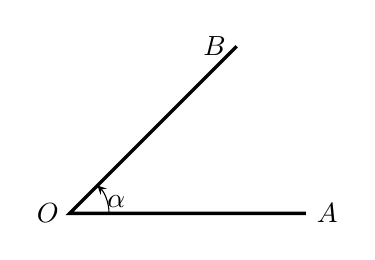
\begin{tikzpicture}[>=stealth]
\draw[very thick](45:3)node[left]{$B$}--(0,0)node[left]{$O$}--(3,0)node[right]{$A$};
\draw[->](.5,0) arc (0:45:.5)node[below right]{$\alpha$};
\end{tikzpicture}    
\captionof{figure}{}
\end{minipage}\hfill
\begin{minipage}{.4\textwidth}
    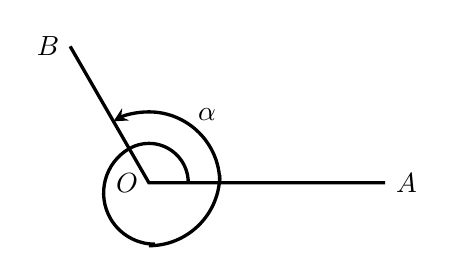
\begin{tikzpicture}[>=stealth]
\draw[very thick](120:2)node[left]{$B$}--(0,0)node[left]{$O$}--(3,0)node[right]{$A$};
\draw[very thick](.5,0) arc (0:120:.5);
\draw[very thick](120:.5) arc (120:270:.65);
\draw[very thick](270:.8) arc (270:360:.9);
\draw[->, very thick](.9,0) arc (0:120:.9);
\node at (60:1)[right]{$\alpha$};
\end{tikzpicture}    
\captionof{figure}{}
    \end{minipage}

在实际生活中,角的形成有两种相反的旋转方向。除了上述逆时针方向外,按顺时针方向旋转也可以形成角。为了区别这两种旋转方向,我们把按逆时针旋转形成的角叫做\textbf{正角}。把按顺时针方向旋转形成的角叫做\textbf{负角}。如图1.6中,以$OA$为始边的角$\alpha=240^{\circ}$,$\beta=-120^{\circ}$, $\gamma=-585^{\circ}$.特别地,当射线$OA$没有做任何旋转时,我们也认为这时形成了一个角,并把这个角叫做\textbf{零角}。当射线逆时针旋转不足一圈时所形成的角叫做\textbf{周内角}。显然周内角的取值范围是$[0,2\pi)$。角的概念经这样推广后,它包括任意大小的正角、负角和零角。

\begin{figure}[htp]
    \centering
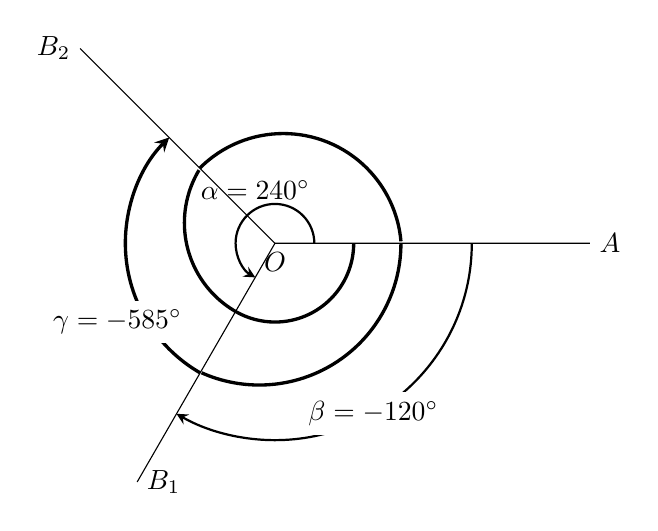
\begin{tikzpicture}[>=stealth]
\draw(-120:3.5)node[right]{$B_1$}--(0,0)node[below]{$O$}--(4,0)node[right]{$A$};
\draw(0,0)--(135:3.5)node[left]{$B_2$};
\draw[->, thick](2.5,0) arc  (0:-120:2.5);
\node at (-60:2.5)[fill=white]{$\beta=-120^{\circ}$};
\draw[->, thick](.5,0) arc  (0:240:.5);
\node at (120:.5)[above]{$\alpha=240^{\circ}$};
\draw[very thick](1,0) arc (0:-120:1);
\draw[very thick](-120:1) arc (-120:-180-31:1.3);
\draw[very thick](135:1.35) arc (135:5:1.5);
\draw[very thick](1.6,0) arc (0:-114:1.8);
\draw[very thick, ->](-120:1.9) arc (-120:-180-45:1.9);
\node at (-2,-1)[fill=white]{$\gamma=-585^{\circ}$};
\end{tikzpicture}
    \caption{}
\end{figure}

在用弧度制度量角时,正角的弧度数为正数,负角的弧度数是负数,零角的弧度数是零。即\textbf{角的弧度数集合与实数集合$\R$可以建立一一对应的关系}:每一个角的弧度数对应唯
一确定的实数,反之,每一个实数对应唯一确定的角的弧度数。

\begin{figure}[htp]
    \centering
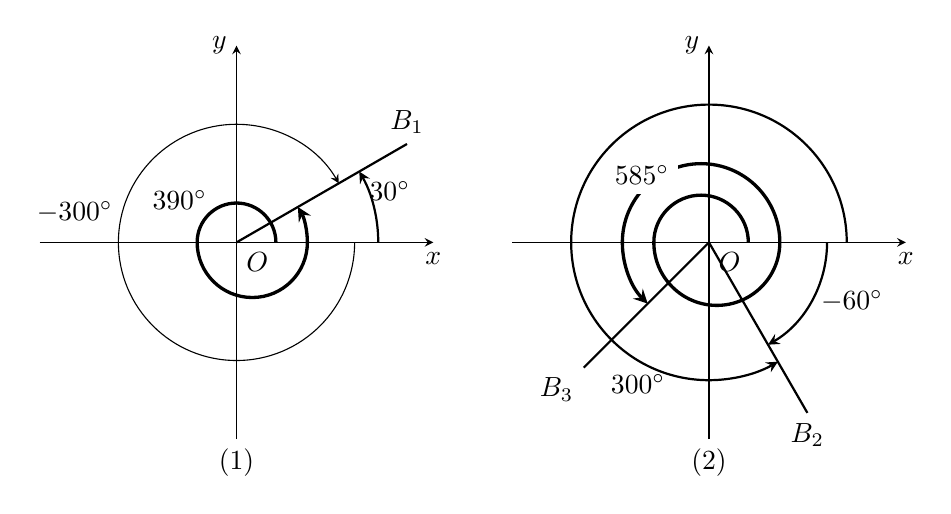
\begin{tikzpicture}[>=stealth]
\begin{scope}
\draw[->](-2.5,0)--(2.5,0)node[below]{$x$};
\draw[->](0,-2.5)node[below]{(1)}--(0,2.5)node[left]{$y$};
\node [below right]{$O$};
\draw[thick](0,0)--(30:2.5)node[above]{$B_1$};
\draw[->](1.5,0) arc (0:-330:1.5);
\node at (165:1.5)[left]{$-300^{\circ}$};
\node at (115:.6)[left]{$390^{\circ}$};
\draw[->, thick](1.8,0) arc (0:30:1.8)node[below right]{$30^{\circ}$};
\draw[very thick](0.5,0) arc (0:180:.5);
\draw[very thick](-.5,0) arc (180:360:.7);
\draw[very thick, ->](.9,0) arc (0:30:.9);
\end{scope}
\begin{scope}[xshift=6cm]
    \draw[->](-2.5,0)--(2.5,0)node[below]{$x$};
\draw[->](0,-2.5)node[below]{(2)}--(0,2.5)node[left]{$y$};
\node [below right]{$O$};
\draw[thick](0,0)--(-60:2.5)node[below]{$B_2$};
\draw[thick](0,0)--(-135:2.25)node[below left]{$B_3$};
\draw[->, thick](1.75,0) arc (0:300:1.75);
\draw[->, thick](1.5,0) arc (0:-60:1.5);
\node at (-30:1.5)[right]{$-60^{\circ}$};
\node at (-120:1.8)[below]{$300^{\circ}$};
\draw[very thick](.5,0) arc (0:180:.6);
\draw[very thick](-.7,0) arc (180:360:.8);
\draw[very thick](.9,0) arc (0:180:1);
\draw[very thick, ->](-1.1,0) arc (180:180+45:1.1) ;
\node at (-.85,.85)[fill=white]{$585^{\circ}$};
\end{scope}
\end{tikzpicture}
    \caption{}
\end{figure}


今后,我们经常在直角坐标系中研究角。使角的顶点与坐标原点重合,始边$OA$与$x$轴正半轴重合(图1.7),让$OA$逆时针或顺时针旋转就可以得到任意大小的角。如果角的终边落在第几象限,就说这个角是第几象限的角(或说这个角属于第几象限)。如图1.7(1)中的角$30^{\circ}$,$390^{\circ}$,$-330^{\circ}$都是第一象限的角;图1.7(2)中的$300^{\circ}$,$-60^{\circ}$的角都是第四象限的角;$585^{\circ}$的角是第三象限的角。如果角的终边落在坐标轴上,就认为这个角不属于任何象限(称这类角为轴上角)。

在图1.7(1)中我们发现:$390^{\circ}$的角与$-330^{\circ}$的角都与$30^{\circ}$的角终边相同。

\begin{thm}{问1}
试把与$30^{\circ}$的角终边相同的一切角的值表示出来。
\end{thm}

很明显,当且仅当$30^{\circ}$加上“周角”的整数倍时,所得到
的角
\begin{equation}
    30^{\circ}+360^{\circ}\cdot k\quad (k\in\Z) \tag{1}
\end{equation}
的终边必定与$30^{\circ}$的角的终边相同。

当$k=0$时,它表示$30^{\circ}$的角;当$k=1$时,它表示$390^{\circ}$的角;当$k=-1$时,它表示$-330^{\circ}$的角,等等。把这一结果写成一般形式有

\begin{thm}
    {定理} 角$\beta$与角$\alpha$终边相同的充要条件是
\[\beta=\alpha+2\pi k\quad (k\in\Z)\]
\end{thm}

特别地,当$\alpha$是一个周内角时,上述结论仍然成立。

\begin{example}
    把下列各角写成周内角加上周角的整数倍的形式:
\begin{multicols}{4}
\begin{enumerate}[(1)]
    \item $855^{\circ}$
    \item $\frac{19\pi}{2}$
    \item $-\frac{16\pi}{3}$
    \item $-1410^{\circ}$
\end{enumerate}
\end{multicols}
\end{example}

\begin{solution}
\begin{enumerate}[(1)]
    \item $855^{\circ}=135^{\circ}+360^{\circ}\x 2$
    \item $\frac{19\pi}{2}=\frac{16\pi+3\pi}{2}=\frac{3\pi}{2}+2\pi\x 4$
    \item $-\frac{16\pi}{3}=\frac{-18\pi+2\pi}{3}=\frac{2\pi}{3}+2\pi\x (-3)$
    \item $-1410^{\circ}=-1440^{\circ}+30^{\circ}=30^{\circ}+360^{\circ}\x (-4)$
\end{enumerate}
\end{solution}

\section*{习题二}
\begin{center}
    \bfseries A
\end{center}

\begin{enumerate}
    \item 把下列度化成弧度:
\begin{multicols}{4}
\begin{enumerate}[(1)]
    \item $18^{\circ }$
    \item $- 120^{\circ }$
    \item $735^{\circ }$
    \item $-12.5^{\circ}$
    \item $10^{\circ}$
    \item $-1080^{\circ}$
    \item $19^{\circ}48^{\prime}$
    \item $-9^{\circ}20^{\prime}$
\end{enumerate}
\end{multicols}
    
\item     把下列弧度化成度。
\begin{multicols}{4}
\begin{enumerate}[(1)]
    \item $- \frac {7\pi }6$
    \item $\frac {\pi} {15}$
    \item $\frac {5\pi} {8}$
    \item $-\frac {8\pi} {3}$
    \item $-5$
    \item $1.4$
    \item $-12\pi$
    \item $-100\pi$
\end{enumerate}
\end{multicols}
\item 把下列角化成“周内角$+$周角的整数倍”的形式。
\begin{multicols}{4}
\begin{enumerate}[(1)]
    \item $-315^{\circ}$
    \item $1200^{\circ}$
    \item $-720^{\circ}$
    \item $-3500^{\circ}$
    \item $\frac{39\pi}{2}$
    \item $-\frac{7\pi}{5}$
    \item $- \frac {76}3\pi$
    \item $- \frac {397}4\pi$
\end{enumerate}
\end{multicols}

\item     下列各组中的两个角的终边是否相同(要简述理由)?
\begin{multicols}{2}
\begin{enumerate}[(1)]
    \item    $3570^{\circ}$与$2130^{\circ}$
    \item $-875^{\circ}$与$565^{\circ}$
    \item $\frac{285\pi}{7}$与$\frac{397\pi}{7}$
    \item $-\frac{11\pi}{4}$与$\frac{25\pi}{4}$
\end{enumerate}
\end{multicols}
\end{enumerate}    

\begin{center}
    \bfseries B
\end{center}

\begin{enumerate}\setcounter{enumi}{4}
    \item 求证:$\alpha$与$\beta$的终边相同$\Longleftrightarrow \beta=\alpha+2k\pi \; (k\in\Z)$
\end{enumerate}


现在,我们研究轴上角和象限中的角的一般形式。

\begin{figure}[htp]
    \centering
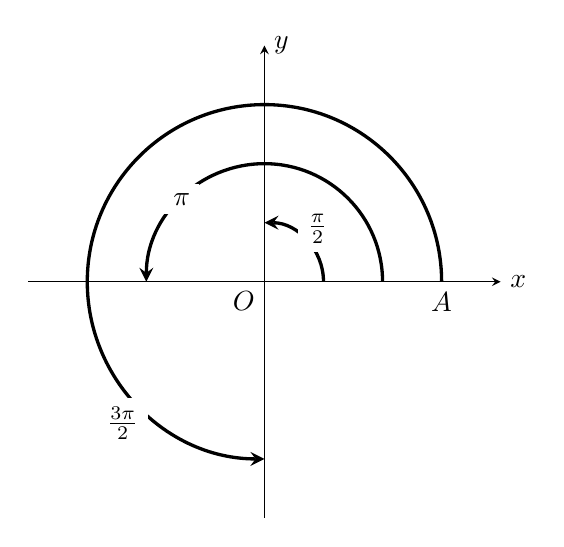
\begin{tikzpicture}[>=stealth, scale=1.5]
    \draw[->](-2,0)--(2,0)node[right]{$x$};
    \draw[->](0,-2)--(0,2)node[right]{$y$};
\node[below left]{$O$};
\draw[->, very thick](.5,0) arc (0:90:.5);
\node at (.45,.45)[fill=white]{$\frac{\pi}{2}$};
\draw[->, very thick](1,0) arc (0:180:1);
\node at (-.7,.7)[fill=white]{$\pi$};
\draw[->, very thick](1.5,0)node[below]{$A$} arc (0:270:1.5); 
\node at (-1.2,-1.2)[fill=white]{$\frac{3\pi}{2}$};
\end{tikzpicture}
    \caption{}
\end{figure}

从图1.8可以看出,终边在轴上的周内角由小到大依次
是
\[0,\quad  \frac{\pi}{2},\quad \pi,\quad \frac{3\pi}{2}\]
将这些角各加上$2k\pi\; (k\in\mathbb{Z})$ 就得到了轴上的所有的角。由此可见:
\begin{itemize}
    \item 终边在$x$轴正半轴上的一切角可以写成$0+2k\pi\; (k\in\mathbb{Z})$;
    \item 终边在$x$轴负半轴上的一切角可以写成$\pi+2k\pi\; (k\in\mathbb{Z})$;
    \item 终边在$y$轴正半轴上的一切角可以写成$\frac{\pi}{2}+2k\pi\; (k\in \Z)$; 
    \item 终边在$y$轴负半轴上的一切角可以写成$\frac{3\pi}{2}+2k\pi\; (k\in \Z)$.
\end{itemize}
进而
\begin{itemize}
    \item 终边在$x$轴上的一切角可写成$k\pi\; (k\in \Z)$;
    \item 终边在$y$轴上的一切角可写成$\frac{\pi}{2}+k\pi\; (k\in \Z)$.
\end{itemize}
再进一步,
\begin{itemize}
    \item 所有的轴上角可写成$\frac{\pi}{2}\cdot k\; (k\in \Z)$.
\end{itemize}

\begin{thm}{思考题}
   终边在$y$轴负半轴上的一切角写成$-\frac{\pi}{2}+2k\pi\; (k\in\Z)$对吗? 
\end{thm}

如果以$\theta_1,\theta_2,\theta_3,\theta_4$分别表示第一、二、三、四象限中的角,那么它们的取值范围是
\[\begin{split}
    0+2k\pi<&\theta_1<\frac{\pi}{2}+2k\pi\\
    \frac{\pi}{2}+2k\pi<&\theta_2<\pi+2k\pi\\
    \pi+2k\pi<&\theta_3<\frac{3\pi}{2}+2k\pi\\
    \frac{3\pi}{2}+2k\pi<&\theta_4<2\pi+2k\pi\\
\end{split}\]
其中:$k\in\Z$.

\begin{note}
    为直观,各象限中的角在写法上通常以周内角为基础,再加上周角的整数倍。
\end{note}

\begin{example}
    第二象限中的角的一半是第几象限中的角?
\end{example}

\begin{solution}

    \noindent
\begin{minipage}{.55\textwidth}
$\because\quad$ 第二象限中的角$\theta_2$满足
\[ \frac{\pi}{2}+2k\pi<\theta_2<\pi+2k\pi\quad (k\in\Z)\]
$\therefore\quad \frac{\pi}{4}+k\pi<\frac{\theta_2}{2}<\frac{\pi}{2}+k\pi\quad (k\in\Z)$

由此式可知:
\begin{itemize}
    \item 当$k$为偶数时,$\frac{\theta_2}{2}$是第一象限中的角;
    \item 当$k$为奇数时,$\frac{\theta_2}{2}$是第三象限中的角(图1.9)。
\end{itemize}

$\therefore\quad $第一象限中的角的半角是第一或第三象限的角.    
\end{minipage}
\hfill
\begin{minipage}{.4\textwidth}
    \centering
\begin{tikzpicture}[>=stealth, scale=1.1]
\draw[->](-2,0)--(2.25,0)node[right]{$x$};
\draw[->](0,-2.5)--(0,2.5)node[left]{$y$};
\node [below right] {$O$};
\fill[pattern=north east lines](0,0)--(0,2.5)--(1.78,1.78)--cycle;
\fill[pattern=north west lines](0,0)--(0,-2.5)--(-1.78,-1.78)--cycle;
\node[fill=white] at (.1,1.5)[right]{\small $k$为偶数};
\node[fill=white] at (-.1,-1.5)[left]{\small $k$为奇数};
\draw[very thick](-1.8,-1.8)node[above]{$\frac{5\pi}{4}$}--(1.8,1.8)node[right]{$\frac{\pi}{4}$};
\end{tikzpicture}
\captionof{figure}{}
\end{minipage}
\end{solution}

\begin{remark}
    这类问题的思考方法是先求出$\frac{\theta}{2}$应满足的关系,再结合图形对整数$k$进行讨论.
\end{remark}

在实际问题中,有时需要计算弧长和扇形的面积。

设圆的半径为$R$(图1.10),$\widearc{AB}$所对的圆心角为$n^{\circ}\; (n>0)$,则:
\begin{itemize}
    \item $\widearc{AB}$的长  \[\ell=\frac{n}{360}\cdot 2\pi R\]
    \item 扇形$\widearc{AOB}$面积 \[S=\frac{n}{360}\cdot \pi R^2\]
    \item 若圆心角为$\alpha$弧度$(\alpha>0)$,则:$\widearc{AB}$的长 \[\ell=\frac{\alpha}{2\pi}\cdot 2\pi R=\alpha R\] (或由公式$\alpha=\ell/R$直接得出)
    \item 扇形$\widearc{AOB}$的面积 \[S=\frac{\alpha}{2\pi}\cdot \pi R^2=\frac{1}{2}\alpha R\cdot R=\frac{1}{2}\ell\cdot R\]
\end{itemize}


\noindent
\begin{minipage}{.45\textwidth}
\centering
\begin{tikzpicture}[>=stealth]
\draw[->](-2.5,0)--(2.5,0)node[right]{$x$};
\draw[->](0,-2.5)--(0,2.5)node[left]{$y$};
\draw[dashed](0,0)node [below right]{$O$} circle (1.5);
\draw[very thick](1.5,0)node[below right]{$A$} arc (0:60:1.5)node[above]{$B$};

\draw(0,0)--(60:1.5);
\draw[->](.5,0)node[above right]{$n^{\circ}$} arc (0:60:.5);
\node at (30:1.75){$\ell$};
\end{tikzpicture}
\captionof{figure}{}
\end{minipage}\hfill
\begin{minipage}{.45\textwidth}
\centering
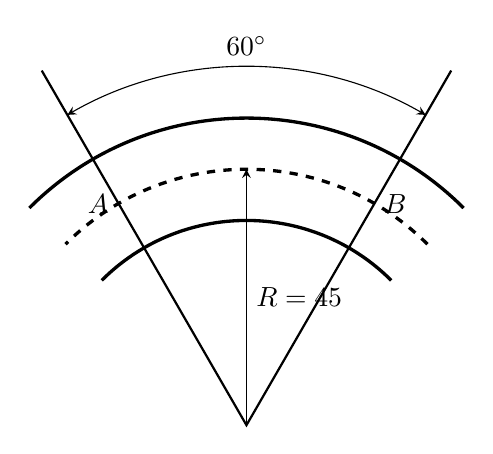
\begin{tikzpicture}[>=stealth,scale=1.3]
\draw[very thick](45:2) arc (45:45+90:2);
\draw[very thick](45:3) arc (45:45+90:3);
\draw[very thick, dashed](45:2.5) arc (45:45+90:2.5);
\draw[thick](120:4)--(0,0)--(60:4);
\draw[->](0,0)--node[right]{$R=45$}(0,2.5);
\node at (60:2.5)[right]{$B$};
\node at (120:2.5)[left]{$A$};
\draw[<->](60:3.5) arc (60:120:3.5);
\node at (0,3.7){$60^{\circ}$};
\end{tikzpicture}
\captionof{figure}{}
\end{minipage}

\begin{example}
    如图1.11,求公路弯道部分$\widearc{AB}$的长(精确到1米,图中的长度是米)
\end{example}

\begin{solution}
$\because\quad \alpha=60^{\circ}=\frac{\pi}{3}$

$\therefore\quad \ell=\alpha R=\frac{\pi}{3}\cdot 45=3.14\x 15\approx 47\text{(米)}$

答:弯道部分$\widearc{AB}$的长约47米.
\end{solution}

\section*{习题三}
\begin{center}
    \bfseries A
\end{center}

\begin{enumerate}
    \item 把下列各角化成“周内角$+$周角的整数倍”的形式,并判定它们各是第几象限中的角或是在哪个坐标轴上的角:
\begin{multicols}{4}
\begin{enumerate}[(1)]
    \item $\frac{155\pi}{4}$
    \item $101\pi$
    \item $\frac{749\pi}{6}$
    \item $-\frac{338\pi}{3}$
    \item $-\frac{59\pi}{2}$
    \item $-\frac{148\pi}{5}$
    \item $-3900^{\circ}$
    \item $-265^{\circ}$
\end{enumerate}
\end{multicols}

\item 与$-\frac{26}{3}\pi$的角终边相同的角的一般形式是\blank,其中最
小的正角是\blank,最大的负角等于\blank.
\item 第四象限中的角的一半是第几象限角?

\item 填表:
\begin{center}
\begin{tabular}{c|c|c|c|c}
  \hline
    角$\theta$所属象限 &\; I\; & \; II\; &\; III&\; IV \\
    \hline
    角$\frac{\theta}{2}$应属的象限 &&&&\\
    \hline
\end{tabular}
\end{center}

\item 已知$(4k+1)\pi<\alpha<(4k+1)\pi+\frac{\pi}{6}\; (k\in\Z)$,
则$\alpha$,$\frac{\alpha}{2}$,$2\alpha$各属第几象限?
\item (口答) \begin{enumerate}[(1)]
\item 第二象限的角一定是钝角吗?
\item $y$轴正半轴上的角一定是直角吗?
\end{enumerate}

\item 
直径是20cm的轮子,每秒钟旋转45弧度,求轮子上一定点经过5秒钟所转过的弧长。
\item 航海罗盘将圆周分成32等份,把一份所对的圆心角的大小分别用度与弧度表示出来。
\item 某种蒸汽机上的飞轮直径为1.2m,每分钟按逆时针方向转300转,求:
\begin{enumerate}[(1)]
\item 飞轮每秒钟转过的弧度数;
\item 轮周上的一点每秒钟经过的弧长。
\end{enumerate}


\item 要在半径$OA=100$cm的圆形金属板上,截取一块$\widearc{AB}$的长为112cm的扇形板,应截取的圆心角$AOB$的度数是多少(精确到$1^{\circ}$)?
\item 已知$1^{\circ}$的圆心角所对的弧长为1m,这个圆的半径是多少?
\item 已知长50cm的弧所对的圆心角为$200^{\circ}$,求该弧所在圆的半径(精确到1cm)。
\item 回忆三角函数的定义,并口述$30^{\circ}$、$45^{\circ}$、$60^{\circ}$各三角函数的值。
\end{enumerate}

\begin{center}
    \bfseries B
\end{center}

\begin{enumerate}\setcounter{enumi}{13}
    \item 写出与$-\frac{5\pi}{3}$终边相同的角的集合$S$,并求出其中属于$[-100\pi, 100\pi)$的角共有多少个?
 \item    如图所示:动点$P$、$Q$同时从点$A(r,0)$出发沿圆周运动。点$P$按逆时针方向
    每秒钟转$\frac{\pi}{3}$弧度,点$Q$按
    顺时针方向每秒钟转$\frac{\pi}{6}$
    弧度,试求点$P,Q$第一次相遇时所用的时间,所在的位置及各自走过的弧长。
\end{enumerate}

\begin{figure}[htp]
    \centering
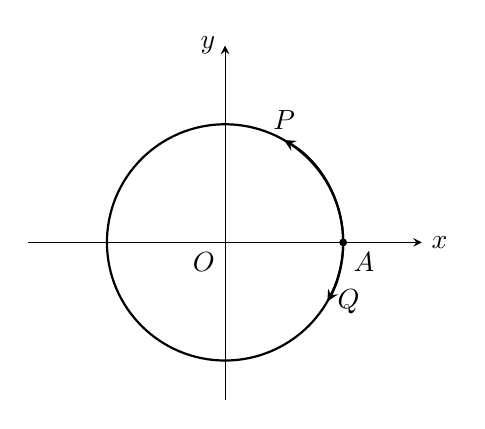
\begin{tikzpicture}[>=stealth]
    \draw[->](-2.5,0)--(2.5,0)node[right]{$x$};
    \draw[->](0,-2)--(0,2.5)node[left]{$y$};
    \draw[ thick](0,0)node [below left]{$O$} circle (1.5);
\draw[ thick, ->](1.5,0) arc (0:60:1.5)node[above]{$P$};
\draw[ thick, ->](1.5,0)node[below right]{$A$} arc (0:-30:1.5)node[right]{$Q$};
\draw[fill](1.5,0) circle(1.2pt);

\end{tikzpicture}
    \caption*{(第15题)}
\end{figure}

\section{任意角三角函数的定义}

\subsection{三角函数的定义}
在初中,大家学过的三角函数是这样定义的:设$P(x,y)$是角$\alpha\; (0\le \alpha<2\pi)$的终边$OB$上异于原点的任一点(图1.12),记$|OP|=r\; (r>0)$,则比值$\frac{y}{r},\; \frac{x}{r},\; \frac{y}{x},\; \frac{x}{y}$都是$\alpha$
的函数,依次记为
\[\sin\alpha=\frac{y}{r},\quad \cos\alpha=\frac{x}{r},\quad \tan\alpha=\frac{y}{x},\quad \cot\alpha=\frac{x}{y}\]

\noindent
\begin{minipage}{.45\textwidth}
\centering
\begin{tikzpicture}[>=stealth]
    \draw[->](-2.5,0)--(2.5,0)node[right]{$x$};
    \draw[->](0,-2)--(0,2.5)node[left]{$y$};
\draw[thick](0,0)node[below left]{$O$}--(120:2.5)node[left]{$B$};
\draw[->](.5,0) arc (0:120:.5);
\node at (.5,.5){$\alpha$};
\draw[dashed](-1.5/2,0)node[below]{$x$}--(-1.5/2, 1.5/2*1.732)node[left]{$P(x,y)$}--(0,1.5/2*1.732)node[right]{$y$};
\node at (-.5,1)[right]{$r$};
\end{tikzpicture}    
\captionof{figure}{}
\end{minipage}
\hfill
\begin{minipage}{.45\textwidth}
\centering
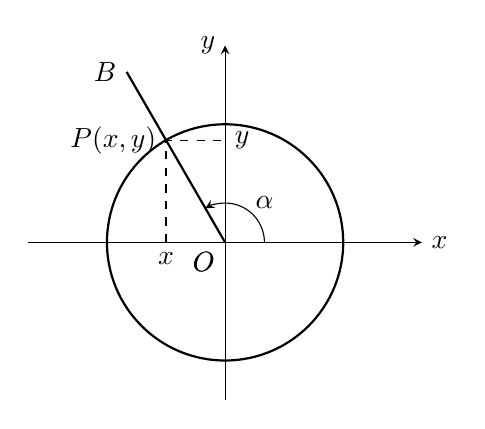
\begin{tikzpicture}[>=stealth]
    \draw[->](-2.5,0)--(2.5,0)node[right]{$x$};
    \draw[->](0,-2)--(0,2.5)node[left]{$y$};
    \draw[ thick](0,0)node [below left]{$O$} circle (1.5);
    \draw[thick](0,0)node[below left]{$O$}--(120:2.5)node[left]{$B$};
    \draw[->](.5,0) arc (0:120:.5);
\node at (.5,.5){$\alpha$};
    \draw[dashed](-1.5/2,0)node[below]{$x$}--(-1.5/2, 1.5/2*1.732)node[left]{$P(x,y)$}--(0,1.5/2*1.732)node[right]{$y$};


\end{tikzpicture}    
\captionof{figure}{}
\end{minipage}


在这个定义中,角$\alpha$的取值范围是$[0,2\pi)$。为今后的需要,现在把它推广到任意角的情况。同时为了研究三角函数的性质更加简便,我们把点$P(x,y)$取在角$\alpha$的终边$OB$与\textbf{单位圆}(以原点为圆心,半径为1的圆)的交点处(图1.13)。应注意,点$P$选在此处不会影响上述四个比值的大小。为叙述方便,今后我们把这个交点叫做角$\alpha$在单位圆上的对应点。于是得到

\begin{thm}
{定义} 设$\alpha$是一个任意角,它的终边$OP$与单位圆相交于点$P(x,y)$,称
\begin{itemize}
    \item $y$为$\alpha$的\textbf{正弦},记为$\sin\alpha=y$;
    \item $x$为$\alpha$的\textbf{余弦},记为$\cos\alpha=x$;
    \item $\frac{y}{x}$为$\alpha$的\textbf{正切},记为$\tan\alpha=\frac{y}{x}$;
    \item $\frac{x}{y}$为$\alpha$的\textbf{余切},记为$\cot\alpha=\frac{x}{y}$;
 \item $\frac{1}{x}$为$\alpha$的\textbf{正割},记为$\sec\alpha=\frac{1}{x}$;
\item $\frac{1}{y}$为$\alpha$的\textbf{余割},记为$\csc\alpha=\frac{1}{y}$.
\end{itemize}
\end{thm}

\begin{note}
当角$\alpha$给定以后,$x$、$y$都被唯一确定,从而上述六个代数式$y$, $x$, $\frac{y}{x}$, $\frac{x}{y}$, $\frac{1}{x}$, $\frac{1}{y}$的值除去有时分母为零以外都是唯一确定的。所以,它们都是$\alpha$的函数。这些函数统称\textbf{三角函数}。
\end{note}

\begin{example}
    求下列各角$\alpha$的六个三角函数值:
\begin{multicols}{4}
\begin{enumerate}[(1)]
    \item $0$
    \item $\frac{\pi}{2}$
    \item $\pi$
    \item $\frac{3\pi}{2}$
\end{enumerate}
\end{multicols}
\end{example}

\begin{solution}
作单位圆,标出这些角对应的点(图1.14)
\begin{figure}[htp]
    \centering
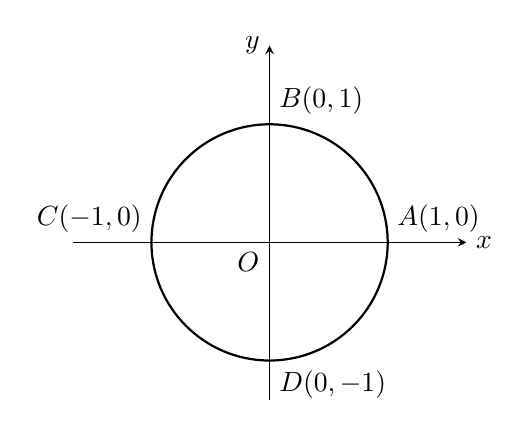
\begin{tikzpicture}[>=stealth]
    \draw[->](-2.5,0)--(2.5,0)node[right]{$x$};
    \draw[->](0,-2)--(0,2.5)node[left]{$y$};
    \draw[ thick](0,0)node [below left]{$O$} circle (1.5);
    \node at (1.5,0)[above right]{$A(1,0)$};
    \node at (-1.5,0)[above left]{$C(-1,0)$};
    \node at (0,1.5)[above right]{$B(0,1)$};
    \node at (0,-1.5)[below right]{$D(0,-1)$};
\end{tikzpicture}
    \caption{}
\end{figure}
\begin{enumerate}[(1)]
    \item $\alpha=0$对应的点为$A(1,0)$,即$x=1$, $y=0$
    
$\therefore\quad \sin 0=0, \; \cos 0=1,\; \tan 0=0,\; \cot0\text{不存在},\; \sec0=1,\; \csc0\text{不存在}$

\item $\alpha=\frac{\pi}{2}$对应的点为$B(0,1)$,即$x=0$, $y=1$
    
$\therefore\quad \sin \frac{\pi}{2}=1, \; \cos \frac{\pi}{2}=0,\; \tan \frac{\pi}{2}\text{不存在},\; \cot\frac{\pi}{2}=0,$

$\sec\frac{\pi}{2}\text{不存在},\; \csc\frac{\pi}{2}=1$

\item $\alpha=\pi$对应的点为$C(-1,0)$,即$x=-1$, $y=0$
    
$\therefore\quad \sin \pi=0, \; \cos \pi=-1,\; \tan \pi=0,\; \cot\pi\text{不存在},\; \sec\pi=-1,\; \csc\pi\text{不存在}$

\item $\alpha=\frac{3\pi}{2}$对应的点为$D(0,-1)$,即$x=0$, $y=-1$
    
$\therefore\quad \sin \frac{3\pi}{2}=-1, \; \cos \frac{3\pi}{2}=0,\; \tan \frac{3\pi}{2}\text{不存在},\; \cot\frac{3\pi}{2}=0,$

$\sec\frac{3\pi}{2}\text{不存在},\; \csc\frac{3\pi}{2}=-1$
\end{enumerate}
\end{solution}

\begin{example}
求下列各角的六个三角函数的值:
\begin{multicols}{4}
\begin{enumerate}[(1)]
    \item $\frac{\pi}{3}$
    \item $\frac{3\pi}{4}$
    \item $\frac{5\pi}{4}$
    \item $\frac{5\pi}{3}$
\end{enumerate}
\end{multicols}
\end{example}

\begin{solution}
作单位圆,标出这些角对应的点(图1.15)
\begin{figure}[htp]
    \centering
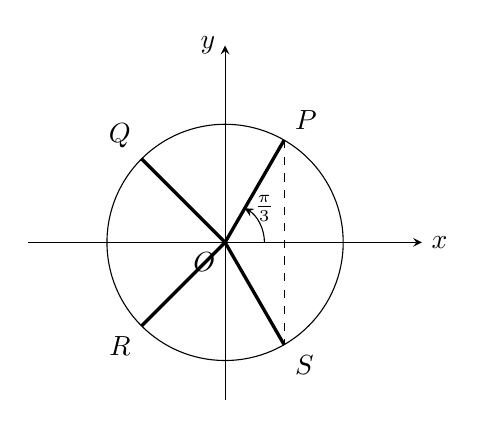
\begin{tikzpicture}[>=stealth]
    \draw[->](-2.5,0)--(2.5,0)node[right]{$x$};
    \draw[->](0,-2)--(0,2.5)node[left]{$y$};
    \draw[](0,0)node [below left]{$O$} circle (1.5);
    \draw[very thick](0,0)-- (60:1.5)node [above right]{$P$};
    \draw[very thick](0,0)-- (135:1.5)node [above left]{$Q$};
    \draw[very thick](0,0)-- (-135:1.5)node [below left]{$R$};
    \draw[very thick](0,0)-- (-60:1.5)node [below right]{$S$};
    \draw[dashed](60:1.5)--(-60:1.5);
    \draw[->](.5,0) arc (0:60:.5)node[right]{\small $\frac{\pi}{3}$};
\end{tikzpicture}
    \caption{}
\end{figure}

\begin{enumerate}[(1)]
    \item $\frac{\pi}{3}$对应的点为$P\left(\frac{1}{2},\frac{\sqrt{3}}{2}\right)$,

$\therefore\quad \sin\frac{\pi}{3}=\frac{\sqrt{3}}{2},\quad \cos\frac{\pi}{3}=\frac{1}{2},\quad \tan\frac{\pi}{3}=\sqrt{3},\quad \cot\frac{\pi}{3}=\frac{\sqrt{3}}{3}$

$\sec\frac{\pi}{3}=2,\quad \csc\frac{\pi}{3}=\frac{2}{3}\sqrt{3}$

\item $\frac{3\pi}{4}$对应的点为$Q\left(-\frac{\sqrt{2}}{2},\frac{\sqrt{2}}{2}\right)$,

$\therefore\quad \sin\frac{3\pi}{4}=\frac{\sqrt{2}}{2},\quad \cos\frac{3\pi}{4}=-\frac{\sqrt{2}}{2},\quad \tan\frac{3\pi}{4}=-1,\quad \cot\frac{3\pi}{4}=-1$

$\sec\frac{3\pi}{4}=-\sqrt{2},\quad \csc\frac{3\pi}{4}=\sqrt{2}$


\item $\frac{5\pi}{4}$对应的点为$R\left(-\frac{\sqrt{2}}{2},-\frac{\sqrt{2}}{2}\right)$,

$\therefore\quad \sin\frac{5\pi}{4}=-\frac{\sqrt{2}}{2},\quad \cos\frac{5\pi}{4}=-\frac{\sqrt{2}}{2},\quad \tan\frac{5\pi}{4}=1,\quad \cot\frac{5\pi}{4}=1$

$\sec\frac{5\pi}{4}=-\sqrt{2},\quad \csc\frac{5\pi}{4}=-\sqrt{2}$

\item $\frac{5\pi}{3}$对应的点为$S\left(\frac{1}{2},-\frac{\sqrt{3}}{2}\right)$,

$\therefore\quad \sin\frac{5\pi}{3}=-\frac{\sqrt{3}}{2},\quad \cos\frac{5\pi}{3}=\frac{1}{2},\quad \tan\frac{5\pi}{3}=-\sqrt{3},\quad \cot\frac{5\pi}{3}=-\frac{\sqrt{3}}{3}$

$\sec\frac{5\pi}{3}=2,\quad \csc\frac{5\pi}{3}=-\frac{2\sqrt{3}}{3}$
\end{enumerate}    
\end{solution}

\subsection{三角函数值的几何表示——三角函数线}
先简介有向线段的概念。

我们知道,坐标轴是规定了方向的直线。线段也可以规
定方向。如图1.16中,在$x$轴上的线段$AB$就可以规定两种相反的方向:以$A$为始点以$B$为终点(记为$\VEC{AB}$),或者以$B$为始点以$A$为终点(记为$\VEC{BA}$)。同样,与$y$轴平行的线段$CD$也
可以规定两种方向:以$C$为始点以$D$为终点(记为$\VEC{CD}$),或者以$D$为始点以$C$为终点(记为$\VEC{DC}$)。如果这条线段的方向与坐标轴的正方向相一致,我们规定用一个正数来表示它,否则就用一个负数来表示它。如上述有向线段可以分别表示成$\VEC{AB}=+3$,$\VEC{BA}=-3$,$\VEC{CD}=-4$,$\VEC{DC}=+4$等。象这样规定了方向的线段,称为\textbf{有向线段}。

现在,我们用有向线段来表示三角函数的值。

\noindent
\begin{minipage}{.45\textwidth}
    \centering
\begin{tikzpicture}[>=stealth, scale=.5]
\draw[->](-4,0)--(5,0)node[below]{$x$};
\draw[->](0,-5)--(0,5)node[left]{$y$};
\foreach \x in {-1,-2,-3,-4,1,2,3,4}
{
    \draw(\x,0)--(\x,.2);
    \draw(0,\x)--(.2,\x);
}
\draw[ultra thick](1,0)node[below]{$A$}--(4,0)node[below]{$B$};
\draw[ultra thick](-2,1)node[left]{$C$}--(-2,-3)node[left]{$D$};
\node [below left]{$O$};

\end{tikzpicture}
\captionof{figure}{}
\end{minipage}\hfill
\begin{minipage}{.45\textwidth}
    \centering
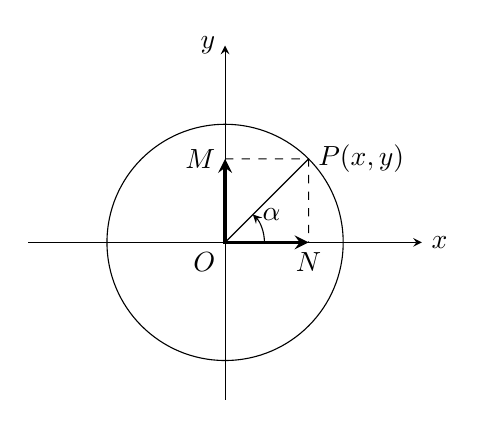
\begin{tikzpicture}[>=stealth]
    \draw[->](-2.5,0)--(2.5,0)node[right]{$x$};
    \draw[->](0,-2)--(0,2.5)node[left]{$y$};
    \draw(0,0)node [below left]{$O$} circle (1.5);
\tkzDefPoints{1.5/0/A, -1.5/0/B, 0/1.5/C, 0/-1.5/D}
\tkzLabelPoints[above left](B)
\tkzLabelPoints[above right](A,C)
\tkzLabelPoints[below right](D)
\draw(0,0)--(45:1.5)node[right]{$P(x,y)$};
\draw[dashed](0,1.5/1.414)node[left]{$M$}--(45:1.5)--(1.5/1.414,0)node[below]{$N$};
\draw[very thick, <->](0,1.5/1.414)--(0,0)--(1.5/1.414,0);
\draw[->](.5,0) arc (0:45:.5)node[right]{$\alpha$};
\end{tikzpicture}
\captionof{figure}{}
\end{minipage}


设角$\alpha$的终边与单位圆相交于$P(x,y)$. 过点$P$分别作$PM\bot y$轴于点$M$,$PN\bot x$轴于点$N$(图1.17)。则有向线段
\[\VEC{OM}=y,\qquad \VEC{ON}=x\]
因此,可以把$\VEC{OM}$和$\VEC{ON}$分别看作是$\sin\alpha=y$和$\cos\alpha=x$的几何形式。今后把$\VEC{OM}$叫做角$\alpha$的\textbf{正弦线},把正弦线所在的直径$\VEC{DC}$叫做\textbf{正弦轴}。同样,把$\VEC{ON}$叫做角$\alpha$的\textbf{余弦线},把余弦线所在直径$BA$叫做\textbf{余弦轴}.

\begin{thm}{思考题1}
    你能画出角$\alpha$的具有代表性的各种情况下的正弦线和余弦线吗?(提示:各有八种情况)
\end{thm}

\begin{thm}
{思考题2} 当角$\alpha$从0增加到$2\pi$时,试根据正弦线$\VEC{OM}$(余弦线$\VEC{ON}$)变化的规律,说出正弦值(余弦值)增、减变化的规律。
   
\end{thm}

现在研究正切值的几何形式。 

角$\alpha$的正切$\tan\alpha=\frac{y}{x}$,欲用一条有向线段表示比值$\frac{y}{x}$是困难的。为此,先作变形:
\begin{equation}
    \tan\alpha=\frac{y}{x}=\frac{\bar y}{1} \tag{*}
\end{equation}
从图1.18可以想到,只要能把$\bar y$表示出来,目标就达到了. 由比例式(*)可以看出,过点$A$作圆的切线$GG'$,连$OP$并延长与$GG'$交于$T$,有
\[\frac{y}{x}=\frac{\VEC{AT}}{OA}=\frac{\VEC{AT}}{1}=\VEC{AT}\]
由此,可以把$\VEC{AT}$叫做角$\alpha$的\textbf{正切线},$\VEC{AT}$所在的圆的切线$GG'$叫做\textbf{正切轴},其方向与$y$轴相同。应该注意的是$\VEC{AT}$的始点是点$A$。终点$T$是$OP$或其反向延长线与正切轴$G'G$的交点。

\begin{figure}[htp]
    \centering
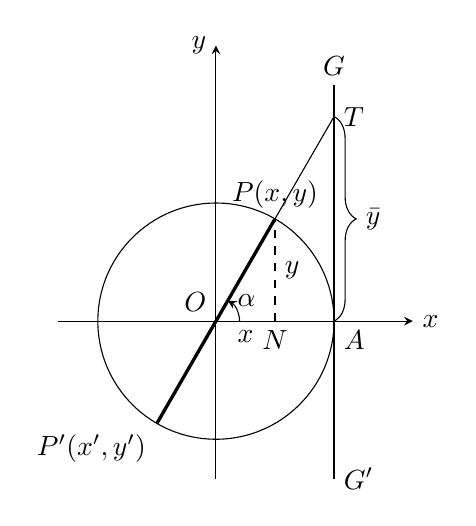
\begin{tikzpicture}[>=stealth]
    \draw[->](-2,0)--(2.5,0)node[right]{$x$};
    \draw[->](0,-2)--(0,3.5)node[left]{$y$};
    \draw(0,0) circle (1.5);
\draw[very thick](-120:1.5)node[below left]{$P'(x',y')$}--(60:1.5)node[above]{$P(x,y)$};
\draw(60:1.5)--(60:3)node[right]{$T$};
\draw(1.5,3)node[above]{$G$}--(1.5,0)node[below right]{$A$}--(1.5,-2)node[right]{$G'$};
\draw[decorate, decoration={brace, amplitude=8pt}](1.5,1.5*1.732)--node[right=8pt]{$\bar y$}(1.5,0);

\node [above left]{$O$};
\draw[->](0.3,0) arc (0:60:.3)node[right]{$\alpha$};
\draw[dashed](1.5/2,0)node[below]{$N$}--node[right]{$y$}(60:1.5);
\node at (1.5/4,0)[below]{$x$};
\end{tikzpicture}
    \caption{}
\end{figure}


\begin{thm}
    {思考题3} 你能画出在各种情况下的具有代表性的正切线吗?(也有八种情况)
\end{thm}


\begin{thm}
    {思考题4} 当角$\alpha$从0增加到$2\pi$时,试根据$\VEC{AT}$的变化规律说出正切值增、减变化的规律。
\end{thm}

\begin{thm}
    {问1} 类比正切线的探寻过程,你能找到余切值的几何形式——余切线吗?
\end{thm}

事实上由
\[\cot\alpha=\frac{x}{y}=\frac{\bar x}{1}\]
由此想到过点$B$作圆的切线$C'C$,连$OP$并延长交$C'C$于$Q$,过$Q$作$QD\bot Ox$轴(图1.19),则$\VEC{OD}=\bar x$,从而
\[\frac{x}{y}=\VEC{OD}=\VEC{BQ}\]
我们把$\VEC{BQ}$叫做角$\alpha$的\textbf{余切线},$\VEC{BQ}$所在的圆的切线叫做\textbf{余切轴},它的方向与$x$轴同向。应该注意,余切线的始点为$B$,终点$Q$则是半径$OP$或其反向延长线与余切轴$CC'$的交点。

\begin{figure}[htp]
    \centering
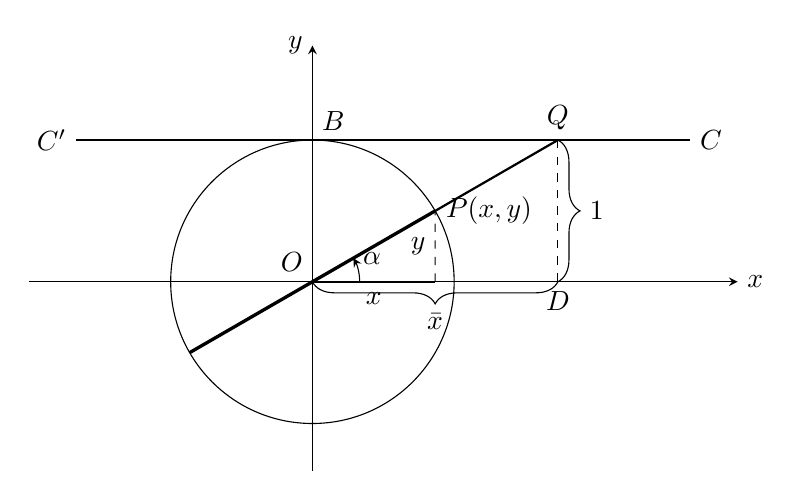
\begin{tikzpicture}[>=stealth, scale=1.2]
    \draw[->](-3,0)--(4.5,0)node[right]{$x$};
    \draw[->](0,-2)--(0,2.5)node[left]{$y$};
    \draw(0,0)node[above left]{$O$} circle (1.5);
\draw[very thick](-150:1.5)--(30:1.5)node[right]{$P(x,y)$};
\draw(-2.5,1.5)node[left]{$C'$}--(4,1.5)node[right]{$C$};
\node at (0,1.5)[above right]{$B$};
\draw[dashed] (1.732*1.5,1.5)node[above]{$Q$}--(1.732*1.5,0)node[below]{$D$};
\draw[thick](1.732*1.5,1.5)--(30:1.5);
\draw[dashed](1.732*1.5/2, 0)--node[left]{$y$}(30:1.5);
\draw[thick](1.732*1.5/2, 0)--node[below]{$x$}(0,0);
\draw[->](.5,0) arc (0:30:.5)node[right]{$\alpha$};
\draw[decorate, decoration={brace, amplitude=8pt}](1.732*1.5,0)--node[below=8pt]{$\bar x$}(0,0);
\draw[decorate, decoration={brace, amplitude=8pt}](1.732*1.5,1.5)--node[right=8pt]{$1$}(1.732*1.5,0);
\end{tikzpicture}
    \caption{}
\end{figure}

\begin{thm}
{思考题5} 请画出在各种情况下具有代表性的余切线,并根据当角$\alpha$从0增加到$2\pi$时,余切线变化的规律说出余切值增、减变化的规律。
\end{thm}

以上,对$\sin\alpha$、$\cos\alpha$、$\tan\alpha$、$\cot\alpha$分别定义了它们的函数线。应明确:每种三角函数的定义及其相应的函数线之间的对应都是数与形的对应。如对$\sin\alpha=y$来说,$y$是它的代数形式,正弦线$\VEC{OM}$是它的几何形式。两种形式各具特色,各有所用,代数形式便于运算,几何形式形象直观。

\section*{习题四}
\begin{center}
    \bfseries A
\end{center}

\begin{enumerate}
    \item 填表:
\begin{center}
\begin{tabular}{c|c|c|c|c|c|c|c}
    \hline
$\alpha$ & 单位圆上 &$\sin\alpha$&$\cos\alpha$&$\tan\alpha$&$\cot\alpha$&$\sec\alpha$&$\csc\alpha$\\
&对应点的坐标是&&&&&& \\
\hline
$\frac{3\pi}{4}$ & $P_1(\qquad \qquad )$&&&&&& \\[1.5ex]
$\frac{5\pi}{4}$ & $P_2(\qquad \qquad )$&&&&&& \\[1.5ex]
$\frac{7\pi}{4}$ & $P_3(\qquad \qquad )$&&&&&& \\[1.5ex]
$\frac{2\pi}{3}$ & $P_4(\qquad \qquad )$&&&&&& \\[1.5ex]
$\frac{4\pi}{3}$ & $P_5(\qquad \qquad )$&&&&&& \\[1.5ex]
$\frac{5\pi}{6}$ & $P_6(\qquad \qquad )$&&&&&& \\[1.5ex]
$\frac{7\pi}{8}$ & $P_7(\qquad \qquad )$&&&&&& \\[1.5ex]
\hline
\end{tabular}
\end{center}    

\item 分别作出下列各角的正弦线、余弦线、正切线、余切线:
\begin{multicols}{4}
\begin{enumerate}[(1)]
    \item $\frac{\pi}{3}$
    \item $\frac{5\pi}{6}$
    \item $-\frac{2\pi}{3}$
    \item $-\frac{13\pi}{6}$
\end{enumerate}
\end{multicols}
\item 以2cm为“单位长”作单位圆,再分别作出角$\alpha$等于$\frac{\pi}{6}$、$\frac{5\pi}{4}$、$\frac{11\pi}{6}$
的正弦线、余弦线、正切线、余切线,量出它们的长度,据此长度把相应的正弦值、余弦值、正切值和余切值(精确到0.1)填入下表之中:
\begin{center}
\begin{tabular}{c|c|c|c|c}
\hline
角$\alpha$ & $\sin\alpha$&$\cos\alpha$&$\tan\alpha$&$\cot\alpha$\\
\hline
$\frac{\pi}{6}$ &&&&\\[1.5ex]
$\frac{5\pi}{4}$ &&&&\\[1.5ex]
$\frac{11\pi}{6}$ &&&&\\[1.5ex]
\hline
\end{tabular}
\end{center}
\end{enumerate}

\begin{center}
    \bfseries B
\end{center}

\begin{enumerate}\setcounter{enumi}{3}
    \item 仍以2cm为“单位长”作单位圆,再作出$\alpha=230^{\circ}$的正弦线、余弦线、正切线、余切线,量出其长,据此写出$\sin\alpha$、$\cos\alpha$、$\tan\alpha$、$\cot\alpha$的值。由此,你能悟出什么道理?
\end{enumerate}

\section{由定义和三角函数线观察三角函数的某些性质}
为了进行三角函数值的计算,本节对三角函数的某些性质先从直观上作初步的探究。

\subsection{定义域}

\noindent
\begin{minipage}{.45\textwidth}
\CTEXindent    根据三角函数的定义(图1.20)
\[\begin{split}
    \sin\alpha=y,&\quad \cos\alpha=x\\ 
    \tan\alpha=\frac{y}{x},&\quad \cot\alpha=\frac{x}{y}\\
    \sec\alpha=\frac{1}{x},&\quad \csc\alpha=\frac{1}{y}
\end{split}\]
可以看出:

对于正(余)弦,不论$\alpha$为何实数,整式$y$、$x$都有意义,

$\therefore\quad \sin\alpha,\; \cos\alpha$的定义域为$\alpha\in\R$;


\end{minipage}\hfill
\begin{minipage}{.45\textwidth}
\centering
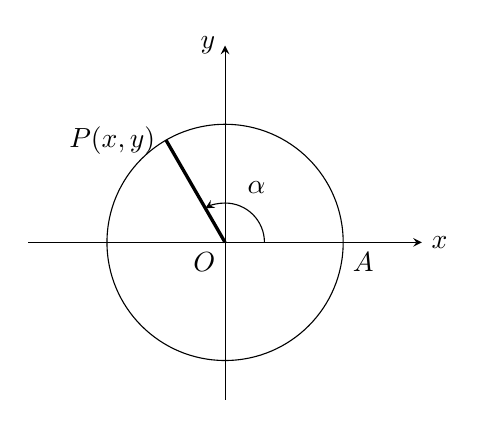
\begin{tikzpicture}[>=stealth]
    \draw[->](-2.5,0)--(2.5,0)node[right]{$x$};
    \draw[->](0,-2)--(0,2.5)node[left]{$y$};
    \draw(0,0)node[below left]{$O$} circle (1.5);
\node at (1.5,0)[below right]{$A$};
\draw[very thick](0,0)--(120:1.5)node[left]{$P(x,y)$};
\draw[->](0.5,0) arc (0:120:.5);
\node at (60:.8){$\alpha$};
\end{tikzpicture}
\captionof{figure}{}
\end{minipage}

对于正切与正割,除去$y$轴上的点以外,分式$\frac{y}{x}$, $\frac{1}{x}$
都有意义,

$\therefore\quad \tan\alpha$的定义域为$\alpha\in\R$ 且$\alpha\ne \frac{\pi}{2}+k\pi\; (k\in\Z)$, 

对于余切与余割,除去$x$轴上的点以外,分式$\frac{x}{y}$, $\frac{1}{y}$都有意义,

$\therefore\quad \cot\alpha,\; \csc\alpha$的定义域为$a\in\R$,且$\alpha\ne k\pi\; (k\in\Z)$.

\subsection{函数值的符号和取值范围(函数的值域)}
从三角函数线的变化规律以及正(余)割的定义可以看出,当角$\alpha$在各自定义域上变化时,其函数值的取值范围如下表所示,其函数值在四个象限中的符号如图1.21所示。
\begin{center}
    \begin{tabular}{c|c|c|c}
\hline
函数名称& 定义式& 定义域& 值域\\
\hline
$\sin\alpha$ & $y$  &  $\alpha\in\R$ &  $[-1,\;1]$\\[1.5ex]
$\cos\alpha$ & $x$  &  $\alpha\in\R$ &  $[-1,\;1]$\\[1.5ex]
$\tan\alpha$ & $\frac{y}{x}$  &  $\alpha\in\R$且$\alpha\ne \frac{\pi}{2}+k\pi\; (k\in\Z)$ &  $(-\infty,\;+\infty)$\\[1.5ex]
$\cot\alpha$ & $\frac{x}{y}$  &  $\alpha\in\R$且$\alpha\ne k\pi\; (k\in\Z)$ &  $(-\infty,\;+\infty)$\\[1.5ex]
$\sec\alpha$ & $\frac{1}{x}$  &  $\alpha\in\R$且$\alpha\ne \frac{\pi}{2}+k\pi\; (k\in\Z)$ &  $(-\infty,-1]\cup[1,+\infty)$\\[1.5ex]
$\csc\alpha$ & $\frac{1}{y}$  &  $\alpha\in\R$且$\alpha\ne k\pi\; (k\in\Z)$ &  $(-\infty,-1]\cup[1, +\infty)$\\[1.5ex]
\hline
    \end{tabular}
\end{center}

\begin{figure}[htp]
    \centering
\begin{tikzpicture}[>=stealth, scale=1.1]
\begin{scope}
    \draw[->](-1.5,0)--(1.5,0)node[right]{$x$};
    \draw[->](0,-1.5)node[below]{$\sin\alpha$与$\csc\alpha$}--(0,1.5)node[left]{$y$};
    \draw(0,0)node[below left]{$O$} circle (1);
\node at (.5,.5){$+$};
\node at (-.5,.5){$+$};
\node at (.5,-.5){$-$};
\node at (-.5,-.5){$-$};
\end{scope}
\begin{scope}[xshift=4cm]
    \draw[->](-1.5,0)--(1.5,0)node[right]{$x$};
    \draw[->](0,-1.5)node[below]{$\cos\alpha$与$\sec\alpha$}--(0,1.5)node[left]{$y$};
    \draw(0,0)node[below left]{$O$} circle (1);
\node at (.5,.5){$+$};
\node at (-.5,.5){$-$};
\node at (.5,-.5){$+$};
\node at (-.5,-.5){$-$};
\end{scope}
\begin{scope}[xshift=8cm]
    \draw[->](-1.5,0)--(1.5,0)node[right]{$x$};
    \draw[->](0,-1.5)node[below]{$\tan\alpha$与$\cot\alpha$}--(0,1.5)node[left]{$y$};
    \draw(0,0)node[below left]{$O$} circle (1);
\node at (.5,.5){$+$};
\node at (-.5,.5){$-$};
\node at (.5,-.5){$-$};
\node at (-.5,-.5){$+$};
\end{scope}
\end{tikzpicture}
    \caption{}
\end{figure}

\subsection{诱导公式}
\subsubsection{$f(\alpha+2k\pi)$与$f(\alpha)$之间的关系}

为叙述方便,以下统一用$f(\alpha)$表示角$\alpha$的六个三角函数。欲求$f(\alpha+2k\pi)$与$f(\alpha)$之关系,只要弄清楚角$\alpha$与$\alpha+2k\pi\; (k\in\Z)$的对应点在单位圆上的位置关系就行了。据1.2节的定理,这两个对应点在单位圆上重合,即它们的直角坐标完全相同。
\[\therefore\quad f(\alpha+2k\pi)=f(\alpha)\]
这样,就得到了

\begin{thm}{公式(一)}
\[\begin{split}
\sin(\alpha+2k\pi)=\sin\alpha   &\qquad  \cos(\alpha+2k\pi)=\cos\alpha \\
\tan(\alpha+2k\pi)=\tan\alpha  &\qquad \cot(\alpha+2k\pi)=\cot\alpha \\
\sec(\alpha+2k\pi)=\sec\alpha  &\qquad \csc(\alpha+2k\pi)=\csc\alpha \\
\end{split}\]
其中,$k\in\Z$.
\end{thm}

由于“$2k\pi\; (k\in\Z)$”是周角的整数倍,这组公式表明:在计算三角函数值的时候,周角的整数倍可以“去掉”。特别地,当$\alpha$是周内角时,这组公式的功能在于:能把周外角的函数化为周内角的函数,从而能简化函数性质的研究和计算。

\subsubsection{$f(-\alpha)$与$f(\alpha)$之间的关系}

$\because\quad $角$\alpha$与$(-\alpha)$的对应点$P(x,y)$与$P'(x',y')$关于$x$轴对称(图1.22)

$\therefore\quad x=x',\quad y=-y'$

从而,得到:

\begin{thm}{公式(二)}
    \[\begin{split}
\sin(-\alpha)=-\sin\alpha   &\qquad  \cos(-\alpha)=+\cos\alpha \\
\tan(-\alpha)=-\tan\alpha  &\qquad \cot(-\alpha)=-\cot\alpha \\
\sec(-\alpha)=+\sec\alpha  &\qquad \csc(-\alpha)=-\csc\alpha \\
\end{split}\]
\end{thm}

这组公式的功能在于:能把负角的函数化为正角的函数,从而能简化函数性质的研究和计算。



\noindent
\begin{minipage}{.45\textwidth}
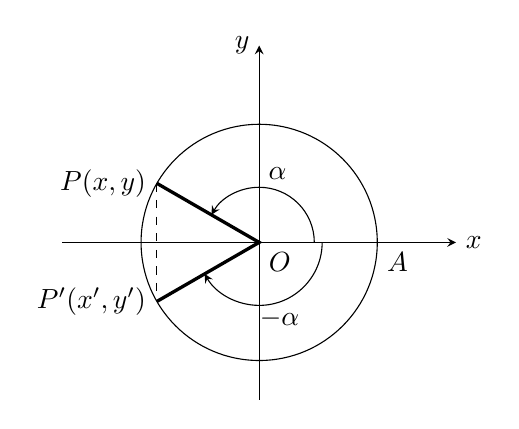
\begin{tikzpicture}[>=stealth]
    \draw[->](-2.5,0)--(2.5,0)node[right]{$x$};
    \draw[->](0,-2)--(0,2.5)node[left]{$y$};
    \draw(0,0)node[below right]{$O$} circle (1.5);
\draw[very thick](150:1.5)node[left]{$P(x,y)$}--(0,0)--(-150:1.5)node[left]{$P'(x',y')$};
\draw[dashed](150:1.5)--(-150:1.5);
\draw[->](.7,0) arc (0:150:.7);
\draw[->](.8,0) arc (0:-150:.8);
\node at (1.5,0)[below right]{$A$};
\node at (75:.9){$\alpha$};
\node at (-75:1){$-\alpha$};
\end{tikzpicture}
\captionof{figure}{}
\end{minipage}\hfill
\begin{minipage}{.45\textwidth}
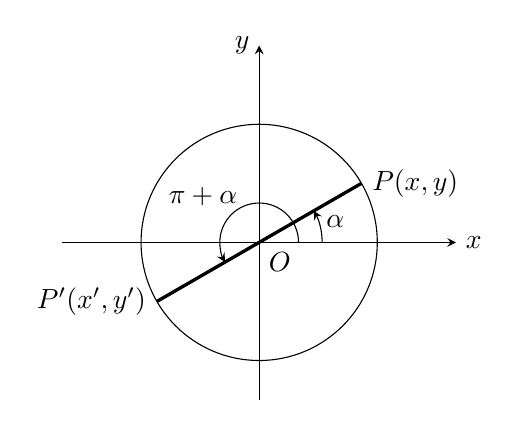
\begin{tikzpicture}[>=stealth]
    \draw[->](-2.5,0)--(2.5,0)node[right]{$x$};
    \draw[->](0,-2)--(0,2.5)node[left]{$y$};
    \draw(0,0)node[below right]{$O$} circle (1.5);
\draw[very thick](210:1.5)node[left]{$P'(x',y')$}--(0,0)--(30:1.5)node[right]{$P(x,y)$};
\draw[->](.5,0) arc (0:210:.5);
\draw[->](.8,0) arc (0:30:.8);
\node at (105:.6)[left]{$\pi+\alpha$};
\node at (15:1){$\alpha$};
\end{tikzpicture}
\captionof{figure}{}
\end{minipage}


\subsubsection{$f(\pi+\alpha)$与$f(\alpha)$之间的关系}
$\because\quad $角$\alpha$与$(\pi+\alpha)$的对应点$P(x,y)$与$P'(x',y')$关于原点对称(图1.23)

$\therefore\quad x=-x',\quad y=-y'$

从而得到:

\begin{thm}{公式(三)}
\[\begin{split}
\sin(\pi+\alpha)=-\sin\alpha   &\qquad  \cos(\pi+\alpha)=-\cos\alpha \\
\tan(\pi+\alpha)=+\tan\alpha  &\qquad \cot(\pi+\alpha)=+\cot\alpha \\
\sec(\pi+\alpha)=-\sec\alpha  &\qquad \csc(\pi+\alpha)=-\csc\alpha \\
\end{split}\]
\end{thm}

这组公式的功能:能把$(\pi+\alpha)$的函数化为$\alpha$的函数,特别,当$\alpha$为锐角时,运用它能把第III象限的角$(\pi+\alpha$)的函数一举化成锐角的函数,从而能把函数简化。要记忆这组公式,关键是记住公式右边的符号——它是视$\alpha$为锐角时原来函数$f(\pi+\alpha)$的值的符号。

\subsubsection{$f(\pi-\alpha)$与$f(\alpha)$之间的关系}
$\because\quad $角$\alpha$与$(-\alpha)$的对应点P与Q关于x轴对称,而$(-\alpha)$与$(-\alpha+\pi)$的对应点$Q$与$P'$关于原点对称,从而$\alpha$与$(-\alpha+\pi)$的对应点$P(x,y)$与$P'(x',y')$关于$y$轴对称(图1.24)

$\therefore\quad 
x=-x',\quad y=y'$

这样,就得到:

\begin{thm}{公式(四)}
    \[\begin{split}
\sin(\pi-\alpha)=+\sin\alpha   &\qquad  \cos(\pi-\alpha)=-\cos\alpha \\
\tan(\pi-\alpha)=-\tan\alpha  &\qquad \cot(\pi-\alpha)=-\cot\alpha \\
\sec(\pi-\alpha)=-\sec\alpha  &\qquad \csc(\pi-\alpha)=+\csc\alpha \\
\end{split}\]
\end{thm}

\begin{thm}{思考题1}
    你能指出公式(四)的功能以及记忆它的方法吗?
\end{thm}

\begin{thm}{思考题2}
    在公式(三)中,以$(-\alpha)$代替$\alpha$,再用公式(二)也能导出公式(四),试试看,这种做法合理吗?
\end{thm}

\noindent
\begin{minipage}{.45\textwidth}
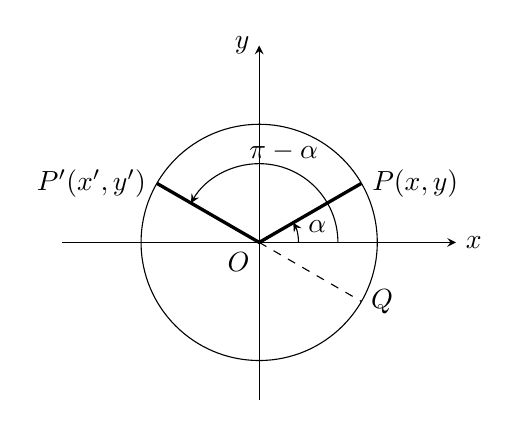
\begin{tikzpicture}[>=stealth]
    \draw[->](-2.5,0)--(2.5,0)node[right]{$x$};
    \draw[->](0,-2)--(0,2.5)node[left]{$y$};
    \draw(0,0)node[below left]{$O$} circle (1.5);
\draw[very thick](150:1.5)node[left]{$P'(x',y')$}--(0,0)--(30:1.5)node[right]{$P(x,y)$};
\draw[dashed](0,0)--(-30:1.5)node[right]{$Q$};
\draw[->](.5,0)node[above right]{$\alpha$} arc (0:30:.5);
\draw[->](1,0) arc (0:150:1);
\node at (75:1.2)[]{$\pi-\alpha$};
\end{tikzpicture}    
\captionof{figure}{}
\end{minipage}\hfill
\begin{minipage}{.45\textwidth}
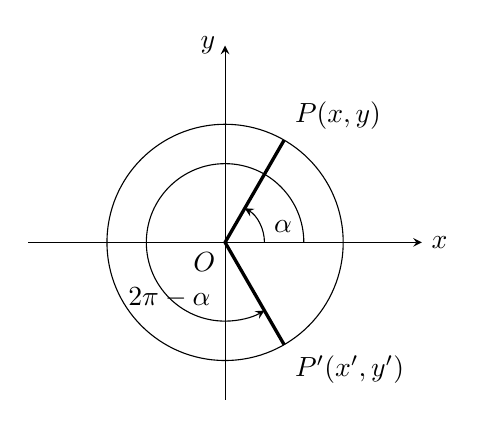
\begin{tikzpicture}[>=stealth]
    \draw[->](-2.5,0)--(2.5,0)node[right]{$x$};
    \draw[->](0,-2)--(0,2.5)node[left]{$y$};
    \draw(0,0)node[below left]{$O$} circle (1.5);
\draw[very thick](60:1.5)node[above right]{$P(x,y)$}--(0,0)--(-60:1.5)node[below right]{$P'(x',y')$};
\draw[->](.5,0)node[above right]{$\alpha$} arc (0:60:.5);
\draw[->](1,0) arc (0:300:1);
\node at (45+180:1){$2\pi-\alpha$};

\end{tikzpicture}    
\captionof{figure}{}
\end{minipage}


\subsubsection{$f(2\pi-\alpha)$与$f(\alpha)$之间的关系}
$\because\quad $角$(2\pi-\alpha)$与$(-\alpha)$的对应点重合,$(-\alpha)$与$\alpha$的对应点关于$x$轴对称,从而$(2\pi-\alpha)$与$\alpha$的对应点$P'(x',y')$与$P(x,y)$关于$x$轴对称(图1.25)

$\therefore\quad x=x',\quad y=-y'$

由此就得到了:
\begin{thm}{公式(五)}
    \[\begin{split}
\sin(2\pi-\alpha)=-\sin\alpha   &\qquad  \cos(2\pi-\alpha)=+\cos\alpha \\
\tan(2\pi-\alpha)=-\tan\alpha  &\qquad \cot(2\pi-\alpha)=-\cot\alpha \\
\sec(2\pi-\alpha)=+\sec\alpha  &\qquad \csc(2\pi-\alpha)=-\csc\alpha \\
\end{split}\]
\end{thm}

对于公式(五),请做出类似于公式(三)的解释。

\begin{thm}
    {思考题} 用公式(一)、(二)能推出公式(五)吗?试试。
\end{thm}

对于上述五组公式概括如下:
\begin{enumerate}
\item 从等号两边式子的结构上看,两边角不同,函数名称相同,符号多数不同,即公式给出了$2k\pi+\alpha\; (k\in\Z)$、$-\alpha$、$\pi\pm\alpha$和$2\pi-\alpha$的三角函数的值等于$\alpha$的同名三角函数值,前面放上把$\alpha$视为锐角时原来函数值的符号;
\item 公式推导的基本方法是利用动点$P(x,y)$与$P'(x',y')$的对称性。从推导过程可见,这些公式在各自函数的定义域上都是恒等式;
\item 联合使用这五组公式,可以把任意角$\alpha$的三角函数的计算通过“去负”(把负角的函数化成正角的函数)、“去周”(把周角的整数倍去掉,化成周内角的函数)、“化锐角”(把$\pi\pm\alpha$、$2\pi-\alpha$的函数化为锐角$\alpha$的函数)的方法,最终诱导到锐角范围加以解决。因此,这五组公式统称\textbf{诱导公式}。
\end{enumerate}

\begin{example}
确定下列函数值的符号:
\begin{multicols}{3}
\begin{enumerate}[(1)]
    \item $\sin\left(-7\frac{1}{3}\pi\right)$
    \item $\cot\frac{29\pi}{3}$
    \item $\sec\left(-\frac{781}{4}\pi\right)$
\end{enumerate}
\end{multicols}
\end{example}

\begin{solution}
\begin{enumerate}[(1)]
    \item $\sin\left(-7\frac{1}{3}\pi\right)=-\sin\left(7\frac{1}{3}\pi\right)=-\sin\left(2\pi\cdot 3+\frac{4}{3}\pi\right)=-\sin\frac{4\pi}{3}>0$

另解:$\sin\left(-7\frac{1}{3}\pi\right)=\sin\left(-7\frac{1}{3}\pi+8\pi\right)=\sin\frac{2\pi}{3}>0$

这个解法表明,对于负角的三角函数值的计算“从右往左”使用公式(一)有时会更加简捷。

\item $\cot\frac{29\pi}{3}=\cot\left(8\pi+\frac{5\pi}{3}\right)=\cot\frac{5\pi}{3}<0$
\item $\sec\left(-\frac{781}{4}\pi\right)=\sec\left(194\pi+\frac{5\pi}{4}\right)=\sec\frac{5\pi}{4}<0$
\end{enumerate}    
\end{solution}

\begin{example}
    给角求函数值:
\begin{multicols}{3}
\begin{enumerate}[(1)]
    \item $\tan\left(-\frac{251\pi}{6}\right)$
    \item $\cos\left(-\frac{52\pi}{3}\right)$
    \item $\csc\left(-\frac{71\pi}{4}\right)$
\end{enumerate}
\end{multicols}
\end{example}

\begin{solution}
\begin{enumerate}[(1)]
    \item $\tan\left(-\frac{251\pi}{6}\right)=\tan\left(-41\frac{5}{4}\pi\right)=\tan\left(-41\frac{5}{6}\pi+42\pi\right)=\tan\frac{\pi}{6}=\frac{\sqrt{3}}{3}$
    \item $\cos\left(-\frac{52\pi}{3}\right)=\cos\frac{52\pi}{3}=\cos\left(16\pi+\pi+\frac{\pi}{3}\right)=\cos\left(\pi+\frac{\pi}{3}\right)=-\cos\frac{\pi}{3}=-\frac{1}{2}$
    \item $\csc\left(-\frac{71\pi}{4}\right)=\csc\left(-17\frac{3}{4}\pi+18\pi\right)=\csc\frac{\pi}{4}=\frac{1}{\sin\frac{\pi}{4}}=\sqrt{2}$
\end{enumerate}
\end{solution}


\section*{习题五}
\begin{center}
    \bfseries A
\end{center}

\begin{enumerate}
    \item 确定下列函数值的符号:
\begin{multicols}{2}
\begin{enumerate}[(1)]
    \item $\cos\frac{16}{5}\pi$
    \item $\cot\left(-\frac{17\pi}{8}\right)$
    \item $\sin\left(\frac{-4\pi}{3}\right)$
    \item $\sin\left(-\frac{67\pi}{12}\right)$
\end{enumerate}
\end{multicols}

\item 求下列各三角函数的值:
\begin{multicols}{3}
\begin{enumerate}[(1)]
    \item $\tan\frac{19\pi}{3}$
    \item $\cot\left(-\frac{29\pi}{4}\right)$
    \item $\tan\left(-\frac{15\pi}{4}\right)$
    \item $\sec\left(-\frac{11\pi}{3}\right)$
    \item $\csc\left(-\frac{25\pi}{3}\right)$
\end{enumerate}
\end{multicols}

\item 计算:
\begin{enumerate}[(1)]
    \item $\cos\frac{\pi}{3}-\tan\frac{\pi}{4}+\frac{3}{4}\tan^2 \frac{\pi}{6}-\sin\frac{\pi}{6}+\cos^2\frac{\pi}{6}+\sin\frac{3\pi}{2}$
    \item $\sin^4 \frac{\pi}{4}-\cos^2\frac{\pi}{2}+6\tan^2\frac{3\pi}{4}$
    \item $7\cos270^{\circ}+12\sin 0^{\circ}+2\cot 90^{\circ}-8\sec 180^{\circ}$
\end{enumerate}

\item 化简:
\begin{enumerate}[(1)]
    \item $a^2\cos 2\pi-b^2\sin\frac{3\pi}{2}+ab\cos \pi-ab\csc\frac{\pi}{2}$
    \item $m\tan0+n\cos\frac{\pi}{2}-p\sin\pi-q\cos\frac{3\pi}{2}-r\sin 2\pi$
    \item $-p^2\sec180^{\circ}+q^2\sin 90^{\circ}-2pq\cos 0^{\circ}$
\end{enumerate}

\item 根据已知条件计算下式的值:
$$\sin\left(t+\frac{\pi}{4}\right)+2\sin\left(t-\frac{\pi}{4}\right)-4\cos 2t+3\cos\left(t+\frac{3}{4}\pi\right)$$
\begin{multicols}{2}
\begin{enumerate}[(1)]
    \item $t=\frac{\pi}{4}$
    \item $t=\frac{3\pi}{4}$
\end{enumerate}
\end{multicols}

\item 确定下列各函数值的符号:
\begin{multicols}{3}
\begin{enumerate}[(1)]
    \item $\sin7.6\pi$
    \item $\cos 101.2\pi$
    \item $\tan88\frac{1}{5}\pi$
    \item $\tan\left(-\frac{23\pi}{4}\right)$
    \item $\cos\left(-\frac{59}{17}\pi\right)$
    \item $\sin 2$
    \item $\cos 3$
    \item $\tan 4$
    \item $\cot 5$
    \item $\csc 6$
\end{enumerate}
\end{multicols}

\item 确定下列各式的符号:
\begin{enumerate}[(1)]
    \item $\sin\frac{5\pi}{4}\cdot \cos \frac{4\pi}{5}\cdot \tan\frac{11\pi}{6}$
    \item $\frac{\sec\frac{5}{6}\pi\cdot \tan\frac{11}{6}\pi}{\csc\frac{2}{3}\pi}$
\end{enumerate}
\end{enumerate}

\begin{example}
判断角$\alpha$的对应点$P$所在的象限:
\begin{multicols}{2}
\begin{enumerate}[(1)]
    \item $\sin\alpha\cdot \cos\alpha>0$
    \item $\frac{\tan\alpha}{\sec\alpha}<0$
\end{enumerate}
\end{multicols}
\end{example}

\begin{solution}
\begin{enumerate}[(1)]
    \item $\because\quad \sin\alpha\cdot \cos\alpha>0$
    
$\therefore\quad \sin\alpha$与$\cos\alpha$同号。
由图1.26知$\alpha$对应的点在第I或第III象限.

\noindent\begin{minipage}{.45\textwidth}
    \centering
\begin{tikzpicture}[>=stealth]
    \draw[->](-2.5,0)--(2.5,0)node[right]{$x$};
    \draw[->](0,-2)node[below, text width=1.5cm, align=center]{$\sin\alpha$\\$\cos\alpha$}--(0,2.15)node[left]{$y$};
    \draw(0,0)node[below right]{$O$} circle (1.5);
\node at (.6,.6) [text width=1cm, align=center]{$+$\\$+$};
\node at (.6,-.6) [text width=1cm, align=center]{$-$\\$+$};
\node at (-.6,.6) [text width=1cm, align=center]{$+$\\$-$};
\node at (-.6,-.6) [text width=1cm, align=center]{$-$\\$-$};

\end{tikzpicture}
\captionof{figure}{}
\end{minipage}
\hfill \begin{minipage}{.45\textwidth}
    \centering
\begin{tikzpicture}[>=stealth]
    \draw[->](-2.5,0)--(2.5,0)node[right]{$x$};
    \draw[->](0,-2)node[below, text width=1.5cm, align=center]{$\tan\alpha$\\$\sec\alpha$}--(0,2.15)node[left]{$y$};
    \draw(0,0)node[below right]{$O$} circle (1.5);
    \node at (.6,.6) [text width=1cm, align=center]{$+$\\$+$};
    \node at (.6,-.6) [text width=1cm, align=center]{$-$\\$+$};
    \node at (-.6,.6) [text width=1cm, align=center]{$-$\\$-$};
    \node at (-.6,-.6) [text width=1cm, align=center]{$+$\\$-$};

\end{tikzpicture}
\captionof{figure}{}
\end{minipage}
 
\item $\because\quad \frac{\tan\alpha}{\sec\alpha}<0$

$\therefore\quad \tan\alpha$与$\sec\alpha$异号,由由图1.27知$\alpha$对应的点在第III或第IV象限.
\end{enumerate}
\end{solution}

\begin{example}
    已知角的范围和角的函数值,求角:
    \begin{multicols}{2}
\begin{enumerate}[(1)]
\item $\alpha$为周内角,且$\sin\alpha=\frac{1}{2}$,
\item $\alpha$为周内角,且$\cos\alpha=-\frac{1}{2}$,
\item $\alpha$为周内角,且$\tan\alpha=-\sqrt{3}$,
\item $\alpha$为周内角,且$\cot\alpha=-\sqrt{3}$,
\item $\alpha$为第II象限角,且$\cos\alpha=-\frac{\sqrt{3}}{2}$.
\end{enumerate}
\end{multicols}
\end{example}

\begin{solution}
\begin{enumerate}[(1)]
\begin{multicols}{2}
    \item 据$\sin\alpha=\frac{1}{2}$, 
    
    作正弦线$\VEC{OM}=\frac{1}{2}$(图1.28)

    $\because\quad \alpha$是周内角,

$\therefore\quad \alpha_1=\frac{\pi}{6},\quad \alpha_2=\frac{5\pi}{6}.$

\item 据$\cos\alpha=-\frac{1}{2}$, 

作余弦线$\VEC{ON}=-\frac{1}{2}$(图1.29)

$\because\quad \alpha$是周内角,

$\therefore\quad \alpha_1=\frac{2\pi}{3},\quad \alpha_2=\frac{4\pi}{3}.$    
\end{multicols}


\noindent\begin{minipage}{.45\textwidth}
    \centering
\begin{tikzpicture}[>=stealth]
    \draw[->](-2.5,0)--(2.5,0)node[right]{$x$};
    \draw[->](0,-2)--(0,2.15)node[left]{$y$};
    \draw(0,0)node[below right]{$O$} circle (1.5);
\node at (1.5,0)[below right]{$A$};
\draw[very thick](30:1.5)node[right]{$P_1$}--(0,0)--(180-30:1.5)node[left]{$P_2$};
\draw[ultra thick, ->](0,0)--node[left]{$\tfrac{1}{2}$}(0,1.5/2)node[above right]{$M$};
\draw[dashed](180-30:1.5)--(30:1.5);

\end{tikzpicture}
\captionof{figure}{}
\end{minipage}
\hfill \begin{minipage}{.45\textwidth}
    \centering
\begin{tikzpicture}[>=stealth]
    \draw[->](-2.5,0)--(2.5,0)node[right]{$x$};
    \draw[->](0,-2)--(0,2.15)node[left]{$y$};
    \draw(0,0)node[below right]{$O$} circle (1.5);
    \node at (1.5,0)[below right]{$A$};
\draw[very thick](180-60:1.5)node[above left]{$P_1$}--(0,0)--(180+60:1.5)node[below left]{$P_2$};
\draw[ultra thick, ->](0,0)--node[above]{$\tfrac{1}{2}$}(-1.5/2,0)node[above left]{$N$};
\draw[dashed](180-60:1.5)--(180+60:1.5);

\end{tikzpicture}
\captionof{figure}{}
\end{minipage}


\noindent\begin{minipage}{.45\textwidth}
    \centering
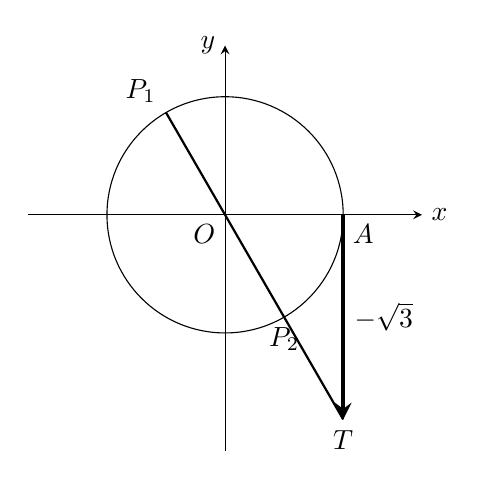
\begin{tikzpicture}[>=stealth]
    \draw[->](-2.5,0)--(2.5,0)node[right]{$x$};
    \draw[->](0,-3)--(0,2.15)node[left]{$y$};
    \draw(0,0)node[below left]{$O$} circle (1.5);
\node at (1.5,0)[below right]{$A$};
\draw[ultra thick, ->](1.5,0)--node[right]{$-\sqrt{3}$}(1.5, -1.5*1.732)node[below]{$T$};
\draw[thick](120:1.5)node[above left]{$P_1$}--(-60:1.5)node[below]{$P_2$}--(1.5, -1.5*1.732);
\end{tikzpicture}
\captionof{figure}{}
\end{minipage}
\hfill \begin{minipage}{.45\textwidth}
    \centering
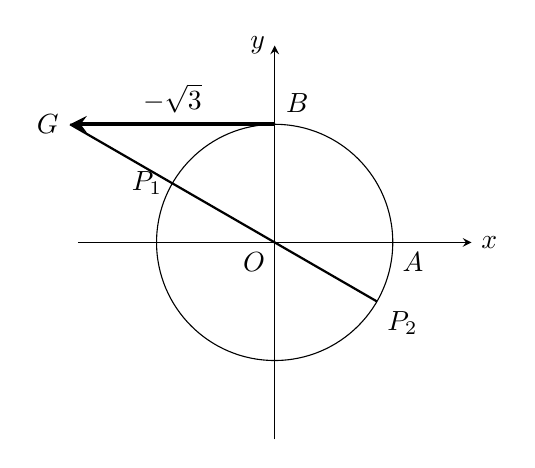
\begin{tikzpicture}[>=stealth]
    \draw[->](-2.5,0)--(2.5,0)node[right]{$x$};
    \draw[->](0,-2.5)--(0,2.5)node[left]{$y$};
    \draw(0,0)node[below left]{$O$} circle (1.5);
    \node at (1.5,0)[below right]{$A$};
    \draw[ultra thick, ->](0,1.5)node[above right]{$B$}--node[above]{$-\sqrt{3}$}(-1.5*1.732,1.5)node[left]{$G$};
\draw[thick](-30:1.5)node[below right]{$P_2$}--(150:1.5)node[left]{$P_1$}--(-1.5*1.732,1.5);
\end{tikzpicture}
\captionof{figure}{}
\end{minipage}


\begin{multicols}{2}
\item 据$\tan\alpha=-\sqrt{3}$, 
    
    作正切线$\VEC{AT}=-\sqrt{3}$(图1.30)

    $\because\quad \alpha$是周内角,

$\therefore\quad \alpha_1=\frac{2\pi}{3},\quad \alpha_2=\frac{5\pi}{3}.$

\item 据$\cot\alpha=-\sqrt{3}$, 

作余切线$\VEC{BG}=-\sqrt{3}$(图1.31)

$\because\quad \alpha$是周内角,

$\therefore\quad \alpha_1=\frac{5}{6}\pi,\quad \alpha_2=\frac{11}{6}\pi.$    
\end{multicols}


\noindent\begin{minipage}{.45\textwidth}
\item 据$\cos\alpha=-\frac{\sqrt{3}}{2}$, 
    
作余弦线$\VEC{ON}=-\frac{\sqrt{3}}{2}$(图1.32)

$\because\quad \alpha$为第II象限角,可先求出周内角$\alpha_1=\frac{5}{6}\pi$,从而
\[\alpha=\frac{5}{6}\pi+2k\pi \quad  (k\in\Z)\]
\end{minipage}
\hfill \begin{minipage}{.45\textwidth}
    \centering
\begin{tikzpicture}[>=stealth]
    \draw[->](-2.5,0)--(2.5,0)node[right]{$x$};
    \draw[->](0,-2.15)--(0,2.15)node[left]{$y$};
    \draw(0,0)node[below right]{$O$} circle (1.5);
    \draw[ultra thick, ->](0,0)--node[below]{$-\tfrac{\sqrt{3}}{2}$}(-1.5/2*1.732,0)node[below]{$N$};
    \draw[dashed](-1.5/2*1.732,0)--(150:1.5);
\draw[thick](180-30:1.5)node[left]{$P$}--(0,0);
\draw[->](.5,0) arc (0:150:.5);
\node at (150/2:.7){$\alpha$};
\end{tikzpicture}
\captionof{figure}{}
\end{minipage}
\end{enumerate}    
\end{solution}

\begin{remark}
这类问题的解题步骤概括为:
\begin{enumerate}
    \item  据函数值,先画出相应的函数线;
    \item  据函数线,定出相应角的对应点(一般有两个);
    \item  据对应点写出相应的周内角(角的特解);
    \item  由“特解$+2k\pi\; (k\in\Z)$”得到角的通解。
\end{enumerate}
\end{remark}

\section*{习题六}

\begin{center}
    \bfseries A
\end{center}

\begin{enumerate}
    \item 根据下列条件,确定$\alpha$属于哪个象限内的角?
 \begin{multicols}{2}
\begin{enumerate}[(1)]
    \item $\sin\alpha<0$且$\cos\alpha>0$
    \item $\sec\alpha<0$且$\cot\alpha<0$
    \item $\sin\alpha\cdot \tan\alpha>0$
    \item $\cos\alpha\cdot \tan\alpha<0$
    \item $\frac{\sin\alpha}{\cot\alpha}>0$
    \item $\sin\alpha\cdot \cos\alpha>0$
\end{enumerate}
 \end{multicols}
 \item    指出下列情况下,$\alpha$的对应点$P$的位置:
 \begin{multicols}{2}
\begin{enumerate}[(1)]
    \item $|\sin\alpha|=\sin\alpha$
    \item $|\cos\alpha|=-\cos\alpha$
    \item $\sin\alpha\cdot \cos\alpha=0$
\end{enumerate}
 \end{multicols}
 \item    求适合下列条件的周内角:
 \begin{multicols}{2}
\begin{enumerate}[(1)]
    \item $\sin\alpha=-\frac{\sqrt{3}}{2}$
    \item $\cos\alpha=-\frac{\sqrt{2}}{2}$
    \item $\tan\alpha=-1$
    \item $\cot\alpha=\sqrt{3}$
\end{enumerate}
 \end{multicols}
 \item    求满足下列条件的角:
 \begin{multicols}{2}
\begin{enumerate}[(1)]
    \item $\cos\alpha=\frac{\sqrt{3}}{2}$,且$\frac{3\pi}{2}<\alpha<2\pi$
    \item $\sin\alpha=-\frac{1}{2}$,且$\pi<\alpha<\frac{3\pi}{2}$
    \item $\cot\alpha=1$,且$\pi<\alpha<\frac{3\pi}{2}$
    \item $\tan\alpha=-\frac{\sqrt{3}}{3}$,且$-2\pi<\alpha<2\pi$
\end{enumerate}
 \end{multicols}

\item 求满足下列条件的角$\alpha$的集合
\begin{multicols}{2}
\begin{enumerate}[(1)]
    \item $\cot\alpha+\sqrt{3}=0$
    \item $\cos(\pi-\alpha)=-\frac{\sqrt{3}}{2}$
    \item $2\sin^2\alpha =1$
\end{enumerate}
\end{multicols}
\end{enumerate}

\begin{center}
    \bfseries B
\end{center}

\begin{enumerate}\setcounter{enumi}{5}
    \item 把圆心角为下列弧度的对应点标在单位圆上:
    $$\alpha _{1}= 1,\quad \alpha _{2}= 2,\quad \alpha _{3}= 3,\quad \alpha _{4}= 4,\quad \alpha _{5}= 5$$
    \item 根据下列条件作出相应的函数线,再用量角器量出相应的周内角$\alpha$:
\begin{multicols}{3}
\begin{enumerate}[(1)]
    \item $\tan\alpha=-2$
    \item $\cos\alpha=-0.4$
    \item $\cot\alpha=-4$
\end{enumerate}
\end{multicols}
\end{enumerate}

\section{同角函数的基本关系}
\begin{thm}
    {问1}
    根据任意角三角函数的定义
\[\begin{split}
    \sin\alpha=y,&\quad \tan\alpha=\frac{y}{x},\quad \sec\alpha=\frac{1}{x}\\
\cos\alpha=x,&\quad \cot\alpha=\frac{x}{y},\quad \csc\alpha=\frac{1}{y}\\
\end{split}\]
参照图1.33,你能发现同一个角$\alpha$的六个三角函数之间的关系吗?
\end{thm}

\noindent 
\begin{minipage}{.45\textwidth}
\CTEXindent
从六个定义的表达式可以看出:
\begin{enumerate}[(1)]
    \item 三个倒数关系
\[\begin{cases}
    \sin\alpha\cdot \csc\alpha=1\\
    \cos\alpha\cdot \sec\alpha=1\\
    \tan\alpha\cdot \cot\alpha=1\\
\end{cases}\]
    \item 三个平方关系
\[\begin{cases}
    \sin^2\alpha+\cos^2\alpha=1\\
    1+\tan^2\alpha =\sec^2\alpha\\
    1+\cot^2\alpha=\csc^2\alpha
\end{cases}\]
\end{enumerate}
\end{minipage}\hfill
\begin{minipage}{.45\textwidth}
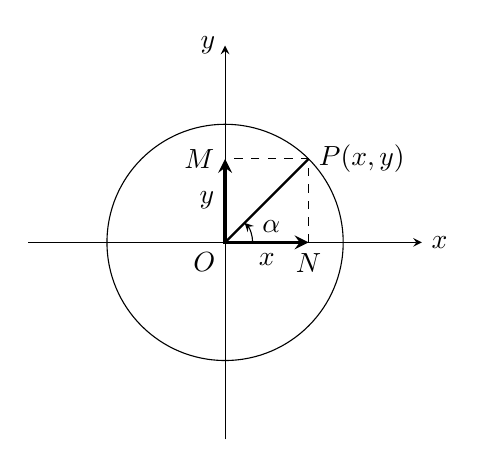
\begin{tikzpicture}[>=stealth]
    \draw[->](-2.5,0)--(2.5,0)node[right]{$x$};
    \draw[->](0,-2.5)--(0,2.5)node[left]{$y$};
    \draw(0,0)node[below left]{$O$} circle (1.5);   
    \draw[very thick, <->](1.5/1.414,0)node[below]{$N$}--node[below]{$x$}(0,0)--node[left]{$y$}(0,1.5/1.414)node[left]{$M$};
    \draw[thick](0,0)--(45:1.5)node[right]{$P(x,y)$};
\draw[dashed](1.5/1.414,0)--(1.5/1.414,1.5/1.414)--(0,1.5/1.414);
\draw[->](.35,0)node[above right]{$\alpha$} arc (0:45:.35);
\end{tikzpicture}
\captionof{figure}{}
\end{minipage}

\begin{enumerate}[(1)]
\setcounter{enumi}{2}    
\item 六个乘积关系
\[\begin{cases}
    \sin\alpha =\tan\alpha  \cdot \cos\alpha \xrightarrow[]{\text{商关系}}\tan\alpha=\frac{\sin\alpha}{\cos\alpha}\\
    \cos\alpha =\cot\alpha  \cdot \sin\alpha \xrightarrow[]{\text{商关系}}\cot\alpha=\frac{\cos\alpha}{\sin\alpha}\\
    \tan\alpha=\sin\alpha\cdot \sec\alpha\\
    \cot\alpha=\cos\alpha\cdot \csc\alpha\\
    \sec\alpha=\tan\alpha\cdot \csc\alpha\\
    \csc\alpha=\cot\alpha\cdot \sec\alpha
\end{cases}\]
\end{enumerate}

\begin{note}
\begin{enumerate}
    \item 公式的发现及证明
    
    根据三角函数定义的表达式容易发现并证明这些公式;
    \item 公式适用的条件
    
    每个公式都是其定义域上的恒等式,即只要角$\alpha$使等号两边的函数都有意义,等式就成立。今后凡说到“恒等式”都是指这个意思;

    \item  公式的实质及功能
    
    三组公式反映了同一个角$\alpha$的六个三角函数之间的关系,通常称作\textbf{同角函数的基本公式}。在三角函数式的恒等变形(又称三角变换)中有着广泛的应用。这里要注意:“同角”应作
    广义的理解,如$3\alpha$与$3\alpha$是同角,$\left(5\alpha+\frac{\pi}{3}\right)$与$\left(5\alpha+\frac{\pi}{3}\right)$也是同角;
    \item 公式的简记法
    
    利用图1.34可以巧妙地记住这些公式(“形象记忆法”)

\begin{figure}[htp]
    \centering
\begin{tikzpicture}
\coordinate(O) at (0,0);
\foreach \x/\y in {0/F,1/A,2/B,3/C,4/D,5/E}
{
    \coordinate (\y) at (\x*60:1.5);
    \draw[very thick](O)--(\y);
}    
\draw[very thick](F)--(A)--(B)--(C)--(D)--(E)--cycle;

\draw[pattern=north east lines](O)--(A)node[above]{$\cos\alpha$}--(B)node[above]{$\sin\alpha$};
\draw[pattern=north east lines](O)--(C)node[left]{$\tan\alpha$}--(D)node[below]{$\sec\alpha$};
\draw[pattern=north east lines](O)--(E)node[below]{$\csc\alpha$}--(F)node[right]{$\cot\alpha$};
\draw[fill=white, very thick]node{1} circle(.35);
\end{tikzpicture}
    \caption{}
\end{figure}

\begin{itemize}
    \item 
    $\text{倒数关系}\xleftrightarrow[]{\text{对应}}\text{三条对角线}$(每条对角线两端的函数成倒数关系);

    \item  $\text{平方关系}\xleftrightarrow[]{\text{对应}}\text{三个倒三角形(阴影所示)}$(倒三角形中,上边两顶点的函数的平方和等于下边顶点上函数的平方);

\item $\text{乘积关系}\xleftrightarrow[]{\text{对应}}\text{相邻三顶点}$(每个顶点上的函数等于相邻两顶点上函数的乘积)。
\end{itemize}
\end{enumerate}
\end{note}

\begin{example}
已知$\sin\alpha=\frac{4}{5}$,$\alpha$是第II象限角,求$\alpha$的其余三角函数值。
\end{example}

\begin{analyze}
图1.34是基本公式的总汇,利用它解这类题是很方便的。
\end{analyze}


\begin{solution}
由$\sin\alpha=\frac{4}{5}\Rightarrow \csc\alpha=\frac{5}{4}$(图1.35)(以下出路在于抓住一个“倒三角形”),

由$\sin^2\alpha+\cos^2\alpha=1$,$\alpha\in $ II象限$\Rightarrow \cos\alpha<0$

$\therefore\quad \cos\alpha=-\sqrt{1-\sin^2\alpha}=-\sqrt{1-\left(\frac{4}{5}\right)^2}=-\frac{3}{5}\Rightarrow \sec\alpha=-\frac{5}{3}$

(以下利用乘积关系)
\[\tan\alpha=\sin\alpha\cdot \sec\alpha=\frac{4}{5}\cdot \left(-\frac{5}{3}\right)=-\frac{4}{3}\Rightarrow \cot\alpha=-\frac{3}{4}\]
\end{solution}

\begin{minipage}{.45\textwidth}
    \centering
\begin{tikzpicture}
\coordinate(O) at (0,0);
\foreach \x/\y in {0/F,1/A,2/B,3/C,4/D,5/E}
{
    \coordinate (\y) at (\x*60:1.5);
    \draw[very thick](O)--(\y);
}    
\draw[very thick](F)--(A)--(B)--(C)--(D)--(E)--cycle;

\draw[pattern=north east lines](O)--(A)--(B)node[above]{$\frac{4}{5}$};
\draw[pattern=north east lines](O)--(C)--(D);
\draw[pattern=north east lines](O)--(E)node[below]{$\frac{5}{4}$}--(F);
\draw[fill=white, very thick]node{1} circle(.35);
\end{tikzpicture}
\captionof{figure}{}
\end{minipage}
\hfill
\begin{minipage}{.45\textwidth}
    \centering
\begin{tikzpicture}
\coordinate(O) at (0,0);
\foreach \x/\y in {0/F,1/A,2/B,3/C,4/D,5/E}
{
    \coordinate (\y) at (\x*60:1.5);
    \draw[very thick](O)--(\y);
}    
\draw[very thick](F)--(A)--(B)--(C)--(D)--(E)--cycle;

\draw[pattern=north east lines](O)--(A)node[above]{$-\frac{8}{17}$}--(B);
\draw[pattern=north east lines](O)--(C)--(D)node[below]{$-\frac{17}{8}$};
\draw[pattern=north east lines](O)--(E)--(F);
\draw[fill=white, very thick]node{1} circle(.35);
\end{tikzpicture}
\captionof{figure}{}
\end{minipage}


\begin{example}
已知$\cos\alpha=-\frac{8}{17}$,求$\alpha$的其余三角函数值.
\end{example}

\begin{analyze}
$\alpha$未加限制,由题知$\alpha\in$ II或III象限。可以先做$\alpha\in$ II象限的情况,然后适当改变正、负号就能得出后一种情况。
\end{analyze}

\begin{solution}
\begin{enumerate}[(1)]
    \item 当$\alpha\in$ II象限时(图1.36),由$\cos\alpha=-\frac{8}{17}\Rightarrow\sec\alpha=-\frac{17}{8}$。
利用$\sin^2\alpha+\cos^2\alpha=1$,得:
\[\sin\alpha=+\sqrt{1-\cos^2\alpha}=\sqrt{1-\left(\frac{-8}{17}\right)^2}=\frac{15}{17}\Rightarrow \csc\alpha=\frac{17}{15}\]
\[\tan\alpha=\sin\alpha\cdot \sec\alpha=\frac{15}{17}\left(-\frac{17}{8}\right)=-\frac{15}{8}\Rightarrow\cot\alpha=-\frac{8}{15}\]

\item 当$\alpha\in$ III象限时,
\[\begin{split}
    \sin\alpha=-\frac{15}{17},&\quad \cos\alpha=-\frac{17}{8},\quad \tan\alpha=\frac{15}{8}\\
    \cot\alpha=\frac{8}{15},&\quad \sec\alpha=-\frac{17}{8},\quad \csc\alpha=-\frac{17}{15}
\end{split} \]
\end{enumerate}
    
\end{solution}

\begin{example}
已知$\cot\alpha=m\; (m\ne 0)$,求$\cos\alpha$.
\end{example}

\begin{figure}[htp]
    \centering
\begin{tikzpicture}
\coordinate(O) at (0,0);
\foreach \x/\y in {0/F,1/A,2/B,3/C,4/D,5/E}
{
    \coordinate (\y) at (\x*60:1.5);
    \draw[very thick](O)--(\y);
}    
\draw[very thick](F)--(A)--(B)--(C)--(D)--(E)--cycle;

\draw[pattern=north east lines](O)--(A)node[above]{?}--(B);
\draw[pattern=north east lines](O)--(C)--(D);
\draw[pattern=north east lines](O)--(E)--(F)node[right]{$m$};
\draw[fill=white, very thick]node{1} circle(.35);
\end{tikzpicture}
    \caption{}
\end{figure}

\begin{analyze}
\begin{enumerate}[(1)]
    \item 从图1.37可见:

思路1:$\cot\alpha=m \xrightarrow[]{\text{平方关系}}\csc\alpha\xrightarrow[]{\text{乘积关系}}\cos\alpha$

思路2:$\cot\alpha=m \xrightarrow[]{\text{平方关系}}\csc\alpha\xrightarrow[]{\text{倒数关系}}\sin\alpha\xrightarrow[]{\text{乘积关系}}\cos\alpha$

思路3:$\cot\alpha=m \xrightarrow[]{\text{倒数关系}}\tan\alpha\xrightarrow[]{\text{平方关系}}\sec\alpha\xrightarrow[]{\text{倒数关系}}\cos\alpha$

相比之下,思路1较简捷。

\item 利用平方关系求$\csc\alpha$时,开平方涉及取正、负号.我们把$\csc\alpha$符号相同的象限分作一组(即分I、II象限与III、IV两种情况,这样在表达上较简明。)
\end{enumerate}
\end{analyze}


\begin{solution}
$\because\quad \cot\alpha=m\ne 0$

$\therefore\quad \alpha$的对应点不在坐标轴上。

\begin{enumerate}[(1)]
    \item 当$\alpha\in$ I、II象限时,$\csc\alpha=+\sqrt{1+\cot^2\alpha}=\sqrt{1+m^2}$
    
利用乘积$\cot\alpha=\cos\alpha\cdot \csc\alpha$可得
\[\cos\alpha=\frac{\cot\alpha}{\csc\alpha}=\frac{m}{\sqrt{1+m^2}}=\frac{m\sqrt{m^2+1}}{m^2+1}\]
\item $\alpha\in $III、IV象限时,
$\csc\alpha=-\sqrt{1+\cot^2\alpha}=-\sqrt{1+m^2}$

$\therefore\quad \cos\alpha=\frac{\cot\alpha}{\csc\alpha}=\frac{m}{-\sqrt{1+m^2}}=\frac{-m\sqrt{1+m^2}}{1+m^2}$
\end{enumerate}
\end{solution}
    
\begin{remark}
\begin{enumerate}
    \item 此例的实质是用$\cot\alpha(\ne  0)$去表示$\cos\alpha$,也就是用$\alpha$的某种函数去表示$\alpha$的其余函数。这种表示主要是出于计算上的需要。应该明确,根据同角函数的基本关系,这种表示总是可以实现的。
    \item 以上三例中,思路探寻都是借助图1.34进行的。这个“神奇的正六边形”不仅囊括了同角函数的全套公式,而且形象地展示了它们之间的联系。这就为使用这些公式提供了极大的方便。
    \item 开平方时要先判断$\alpha$的取值范围,把取“$+$”号的分作一组,把取“$-$”号的分作另一组。这可使表达简单明了。
\end{enumerate}
\end{remark}


\begin{example}
    用$\csc\alpha$表示$\sec\alpha$.
\end{example}

\begin{analyze}
从图1.38可以看出

思路1:$\csc\alpha\xrightarrow[]{\text{平方关系}}\cot\alpha\xrightarrow[]{\text{倒数关系}}\tan\alpha\xrightarrow[]{\text{乘积关系}}\sec\alpha$


思路2:$\csc\alpha\xrightarrow[]{\text{倒数关系}}\sin\alpha\xrightarrow[]{\text{平方关系}}\cos\alpha\xrightarrow[]{\text{倒数关系}}\sec\alpha$
\end{analyze}

\begin{figure}[htp]
    \centering
\begin{tikzpicture}
\coordinate(O) at (0,0);
\foreach \x/\y in {0/F,1/A,2/B,3/C,4/D,5/E}
{
    \coordinate (\y) at (\x*60:1.5);
    \draw[very thick](O)--(\y);
}    
\draw[very thick](F)--(A)--(B)--(C)--(D)--(E)--cycle;

\draw[pattern=north east lines](O)--(A)--(B);
\draw[pattern=north east lines](O)--(C)--(D)node[below]{?};
\draw[pattern=north east lines](O)--(E)node[below]{$\csc\alpha=m$}--(F);
\draw[fill=white, very thick]node{1} circle(.35);
\end{tikzpicture}
    \caption{}
\end{figure}


\begin{solution}
要使$\csc\alpha$与$\sec\alpha$有意义,知$\alpha$不是轴上的角。为表达简单,记$\csc\alpha=m\; (m\ne \pm1)$

利用$1+\cot^2\alpha=\csc^2\alpha$,开平方(分两种情况):
\begin{enumerate}[(1)]
    \item 当$\alpha\in$ I、III象限时,$$\cot\alpha=\sqrt{\csc^2\alpha-1}=\sqrt{m^2-1}\ne 0\Rightarrow \tan\alpha=\frac{1}{\sqrt{m^2-1}}$$

    $\therefore\quad \sec\alpha=\tan\alpha\cdot \csc\alpha=\frac{m}{\sqrt{m^2-1}}=\frac{m\sqrt{m^2-1}}{m^2-1}$
    \item 当$\alpha\in$ II、IV象限时,$$\cot\alpha=-\sqrt{-\csc^2\alpha-1}=-\sqrt{m^2-1}\ne 0\Rightarrow \tan\alpha=\frac{-1}{\sqrt{m^2-1}}$$
    
    $\therefore\quad \sec\alpha=\tan\alpha\cdot \csc\alpha=\frac{-m}{\sqrt{m^2-1}}=\frac{-m\sqrt{m^2-1}}{m^2-1}$.
\end{enumerate}
\end{solution}

\section*{习题七}
\begin{enumerate}
    \item 确定下列函数值的符号:
\begin{multicols}{4}
\begin{enumerate}[(1)]
    \item $\sin 4$
    \item $\cos 5$
    \item $\tan 8$
    \item $\cot(-3)$
\end{enumerate}
\end{multicols}

\item 根据下列条件,求$\alpha$的其余函数值:
\begin{multicols}{2}
\begin{enumerate}[(1)]
    \item $\sin\alpha=\frac{1}{2}$,且$\alpha\in $ I象限
    \item $\cos\alpha=-\frac{4}{5}$,且$\alpha\in $ III象限
    \item $\cot\alpha=-\frac{\sqrt{3}}{3}$
    \item $\tan\alpha=\frac{1}{2}$
\end{enumerate}
\end{multicols}

\item \begin{enumerate}[(1)]
    \item 已知$\cos\theta=\frac{12}{13}$,且$\theta\in $ IV象限,求$\sec\theta$, $\tan\theta$
    \item 已知$\sin\alpha=-\frac{1}{3}$,求$\cos\alpha$, $\tan\alpha$
\end{enumerate}

\item \begin{enumerate}[(1)]
    \item 已知$\tan\alpha=\sqrt{3}$, $\pi<\alpha<\frac{3\pi}{2}$,求$\cos\alpha-\sin\alpha$.
    \item 已知$\cos\alpha=\frac{4}{5}$,求$\sec^2\alpha+\csc^2\alpha$.
\end{enumerate}

\item 已知$\sin x=2\cos x$,求角$x$的六个函数值.
\item \begin{enumerate}[(1)]
    \item 已知$\cos\theta\ne 0$,且$\cos\theta\ne \pm 1$,用$\cos\theta$表示$\theta$的其余函数值;
    \item 已知$\tan\alpha\ne 0$,用$\tan\alpha$表示$\sin\alpha$.
\end{enumerate}
\end{enumerate}

\begin{center}
    \bfseries B
\end{center}

\begin{enumerate}\setcounter{enumi}{6}
    \item 已知$\csc\alpha=t$,求$\cos\alpha$.
    \item 已知$\alpha\in (0,2\pi)$,利用三角函数线证明:$|\sin\alpha|+|\cos\alpha|$不可能小于1.
    \item 已知$\alpha$是锐角,利用三角函数线证明$\sin\alpha<\tan\alpha$.
\end{enumerate}

现在集中讲\textbf{三角函数式的化简}。

力求简捷是数学的特征。对一个三角函数式来说,当然希望它的结果要尽量简单:所包含的角应尽量统一成同角,函数种类和运算种类都要尽量少,字母的次数要尽量低,能求值的应求出值,出现根式要化简,这就是对三角函数式“化简”的一般要求。

此外,当涉及到算术平方根的时候,在过程的表达上首先应把
\[\sqrt{a^2}\xrightarrow[]{\text{写成}}|a|\]
然后,再视情况进一步把
\[|a|\xrightarrow[]{\text{写成}}\begin{cases}
    a, & \text{当}a\ge 0\\
    -a, & \text{当}a< 0\\
\end{cases}\]
这种规范的要求,对减少失误是有益的.

\begin{example}
化简:\begin{multicols}{2}
\begin{enumerate}[(1)]
    \item $\frac{\sin\alpha+\cot\alpha}{\tan\alpha+\csc\alpha}$
    \item $\frac{\sin^4\alpha-\cos^4\alpha}{\sin\alpha+\cos\alpha}$
\end{enumerate}
\end{multicols}
\end{example}

\begin{solution}
\begin{enumerate}[(1)]
    \item \begin{align}
     &   \frac{\sin\alpha+\cot\alpha}{\tan\alpha+\csc\alpha} \tag{分析:函数种类多,化为正余弦}\\
     &=\frac{\sin\alpha+\frac{\cos\alpha}{\sin\alpha}}{\frac{\sin\alpha}{\cos\alpha}+\frac{1}{\sin\alpha}} \tag{分子、分母同乘以$\sin\alpha\cos\alpha$}\\
     &=\frac{\sin^2\alpha\cos\alpha+\cos^2\alpha}{\sin^2\alpha+\cos\alpha}=\frac{\cos\alpha(\sin^2\alpha+\cos\alpha)}{\sin^2\alpha+\cos\alpha}=\cos\alpha \nonumber
    \end{align}
\item \[\begin{split}
    \frac{\sin^4\alpha-\cos^4\alpha}{\sin\alpha+\cos\alpha}&=\frac{(\sin^2\alpha+\cos^2\alpha)(\sin^2\alpha-\cos^2\alpha)}{\sin\alpha+\cos\alpha}\\
    &=\frac{(\sin\alpha+\cos\alpha)(\sin\alpha-\cos\alpha)}{\sin\alpha+\cos\alpha}=\sin\alpha-\cos\alpha
\end{split}\]
\end{enumerate}
\end{solution}

\begin{example}
化简: \begin{multicols}{2}
\begin{enumerate}[(1)]
    \item $\sqrt{1-\sin^2 100^{\circ}}$
    \item $\sqrt{\sec^2\alpha -1}$
    \item $\frac{\sec\alpha}{\sqrt{1+\tan^2\alpha}}+\frac{2\tan\alpha}{\sqrt{\sec^2\alpha-1}}$
    \item $\sqrt{\frac{1+\sin\alpha}{1-\sin\alpha}}-\sqrt{\frac{1-\sin\alpha}{1+\sin\alpha}}$ 
    
    ($\alpha\in$ II象限)
\end{enumerate}
\end{multicols}
\end{example}

\begin{solution}
\begin{enumerate}[(1)]
    \item $\sqrt{1-\sin^2 100^{\circ}}=\sqrt{1-\sin^2 80^{\circ}}=\sqrt{\cos^2 80^{\circ}}=|\cos80^{\circ}|=\cos80^{\circ}$
    \item $\sqrt{\sec^2\alpha -1}=\sqrt{\tan^2\alpha}=|\tan\alpha|$
    \item 
\begin{align}
   & \frac{\sec\alpha}{\sqrt{1+\tan^2\alpha}}+\frac{2\tan\alpha}{\sqrt{\sec^2\alpha-1}}\tag{可以看出:$\alpha$是象限中的角}\\
   &=\frac{\sec\alpha}{\sqrt{\sec^2\alpha}}+\frac{2\tan\alpha}{\sqrt{\tan^2\alpha}} \nonumber\\
    &=\frac{\sec\alpha}{|\sec\alpha|}+\frac{2\tan\alpha}{|\tan\alpha|}=\begin{cases}
        3,&  \text{当$\alpha\in $ I象限} \\
        -3,&  \text{当$\alpha\in $ II象限} \\
        1,&  \text{当$\alpha\in $ III象限} \\
        -1,&  \text{当$\alpha\in $ IV象限} \\
    \end{cases}\nonumber
\end{align}
    
\item 
\begin{align}
   & \sqrt{\frac{1+\sin\alpha}{1-\sin\alpha}}-\sqrt{\frac{1-\sin\alpha}{1+\sin\alpha}}\tag{$\alpha\in $ II 象限}\\
   &=\sqrt{\frac{(1+\sin\alpha)^2}{1-\sin^2\alpha}}-\sqrt{\frac{(1-\sin\alpha)^2}{1-\sin^2\alpha}}\tag{这一步至关重要!目的是把被开方式变成完全平方}\\
   &=\sqrt{\frac{(1+\sin\alpha)^2}{\cos^2\alpha}}-\sqrt{\frac{(1-\sin\alpha)^2}{\cos^2\alpha}}\nonumber\\
   &=\frac{1+\sin\alpha}{|\cos\alpha|}-\frac{1-\sin\alpha}{|\cos\alpha|}\tag{由于$\alpha\in$ II象限,所以$\sin\alpha\in(0,1)\Rightarrow 1\pm\sin\alpha>0$}\\
   &=\frac{2\sin\alpha}{|\cos\alpha|}=\frac{2\sin\alpha}{-\cos\alpha}=-2\tan\alpha \nonumber
\end{align}
\end{enumerate}
\end{solution}

\begin{example}
化简:$\frac{\sin(2\pi-\alpha)\tan(\pi+\alpha)\cot(-\alpha-5\pi)}{\cos(\pi-\alpha)\tan(13\pi-\alpha)}$
\end{example}

\begin{analyze}
不用角多而杂,应统一化作$\alpha$.
\end{analyze}

\begin{solution}
\[\begin{split}
\text{原式}&=\frac{-\sin\alpha \cdot \tan\alpha\cdot \cot(-6\pi+\pi-\alpha)}{-\cos\alpha\cdot \tan(12\pi+\pi-\alpha)}\\
&=\frac{-\sin\alpha \cdot \tan\alpha\cdot \cot (\pi-\alpha)}{-\cos\alpha\cdot \tan(\pi-\alpha)}=\frac{\tan^2\alpha (-\cot\alpha)}{-\tan\alpha}\\
&=\tan\alpha\cdot \cot\alpha =1
\end{split}\]
\end{solution}

\begin{example}
已知$\tan\alpha=-\frac{1}{3}$,求下列各式的值:
\begin{multicols}{2}
\begin{enumerate}[(1)]
    \item $f(a)=\frac{2\sin^2\alpha+3\cos^2\alpha}{\sin^2\alpha+\sin\alpha\cos\alpha}$
    \item $g(\alpha)=\sin^2\alpha+2\sin\alpha\cos\alpha-5\cos^2\alpha$
    \item $h(\alpha)=3\sin\alpha-2\cos\alpha$
\end{enumerate}
\end{multicols}
\end{example}

\begin{analyze}
知$\alpha$的一个函数值,求$\alpha$的三角函数式的值的问
    题,就实质而言,乃是用$\alpha$的这个函数值去表示所求三角函数式的问题,寻找这种表示应是解题的关键。

    由于$\cot\alpha=-3$,$\alpha$是一象限中的角,而所求各式都是$\sin\alpha$、$\cos\alpha$的“齐次式”,抓住这一结构特征,问题就不难解决了。

\begin{enumerate}[(1)]
    \item    分子、分母同除以$\sin^2\alpha$,得
\[f(\alpha)=\frac{2+3\cot^2\alpha}{1+\cot\alpha}=\frac{2+3(-3)^2}{1+(-3)}=\frac{29}{-2}=-14\frac{1}{2}\]
\item $g(\alpha)=\frac{\sin^2\alpha+2\sin\alpha\cos\alpha-5\cos^2\alpha}{\sin^2\alpha+\cos^2\alpha}$(以下略)
\item 可以先算$h^2(\alpha)$,再开平方(注意选取“$+$”、“$-$”号).
\end{enumerate}
\end{analyze}

\begin{remark}
这里三个小题的变形技巧都是从$f(\alpha)$, $g(\alpha)$和$h(\alpha)$是$\sin\alpha$、$\cos\alpha$的“齐次式”想到的。这些技巧是处理这类齐次式的通法。
\end{remark}

\section*{习题八}
\begin{center}
    \bfseries A
\end{center}

\begin{enumerate}
\item 口答下列各式的化简结果:
\begin{multicols}{2}
\begin{enumerate}[(1)]
    \item $\cos\theta\cdot \tan\theta$
    \item $(1+\tan^2\theta)\cos^2\alpha$
    \item $\sin^2 190^{\circ}\cdot \csc^2 190^{\circ}$
    \item $\csc^2\theta-\tan\theta\cdot \cot \theta$
    \item $\sec^2 A-\tan^2A-\sin^2A$
    \item $\frac{1}{\sec^2\alpha}+\frac{1}{\csc^2\alpha}$
    \item $\csc\alpha\cdot \tan\alpha\cdot \sec\alpha\cdot \sin\alpha\cdot \cos \alpha \cdot \cot \alpha$
    \item $\cos^2\alpha\cdot \csc^2\alpha+\sin^2\alpha+\cos^2\alpha$
\end{enumerate}
\end{multicols}

\item 化简:
\begin{multicols}{2}
\begin{enumerate}[(1)]
    \item $\frac{\tan\alpha+\cot\alpha}{\sec\alpha\cdot \csc\alpha}$
    \item $\frac{\sin A+\cos A}{\sec A+\csc A}$
    \item $\frac{2\cos^2 \alpha-1}{1-2\sin^2\alpha}$
    \item $\frac{1-\cos^2\alpha}{1-\sin^2\alpha}+\cos\alpha\cdot \sec\alpha$
    \item $(\tan\beta+\cot\beta)^2-(\tan\beta-\cot\beta)^2$
    \item $\cos^2\alpha\cdot \csc^2\alpha+\sin^2\alpha+\cos^2\alpha$
\end{enumerate}
\end{multicols}

\item 化简:
\begin{enumerate}[(1)]
    \item $\sec\theta \cdot \sqrt{1-\sin^2\theta}$(其中$\theta\in $ II象限)
    \item $\sec\alpha\cdot \sqrt{1+\tan^2\alpha}+\tan\alpha\cdot \sqrt{\csc^2\alpha-1}$(其中$\alpha\in $ IV象限)
    \item $\sqrt{\frac{1+\sin\alpha}{1-\sin\alpha}}-\sqrt{\frac{1-\sin\alpha}{1+\sin\alpha}}$(其中$\alpha\in $ III象限)
    \item $\frac{1}{\cos\alpha \sqrt{1+\tan^2\alpha}}+\frac{2\tan\alpha}{\sqrt{\frac{1}{\cos^2\alpha}-1}}$
    \item $\frac{\sqrt{1-2\sin10^{\circ}\cos10^{\circ}}}{\cos10^{\circ}-\sqrt{1-\cos^2 170^{\circ}}}$
    \item $\sqrt{\sec^2\alpha-2\tan\alpha},\quad \left(0\le \alpha<\frac{\pi}{2}\right)$
    \item $\sqrt{\frac{\sec\alpha-1}{\sec\alpha+1}}+\sqrt{\frac{\sec\alpha+1}{\sec\alpha-1}}$(其中$\alpha\in $ III象限)
\end{enumerate}

\item 填空:若$\frac{\cos\theta}{\sqrt{1+\tan^2\alpha}}+\frac{\sin\theta}{\sqrt{1+\cot^2\alpha}}=-1$,则$\theta$是第\underline{\qquad }象限角.
\item \begin{enumerate}[(1)]
    \item 用$\sec\alpha$表示$\frac{\sin^4\alpha-\cos^2\alpha}{\sin^2\alpha-\cos^2\alpha}+(1+\tan^2\alpha)\cos\alpha$
    \item 用$\cot\alpha$表示$\frac{1+\sin^2\alpha}{\sin^2\alpha}+\frac{\cos^2\alpha}{1-\cos^2\alpha}+\frac{1}{\sec^2\alpha-1}$
\end{enumerate}

\item 已知$\tan\alpha=2$,计算:
\begin{multicols}{2}
    \begin{enumerate}[(1)]
    \item $\frac{\sin\alpha+\cos\alpha}{\sin\alpha-\cos\alpha}$
    \item $\frac{1-2\sin^2\alpha}{\sin\alpha\cdot \cos\alpha}$
    \item $\frac{1}{\sin^2\alpha+2\sin\alpha\cdot \cos\alpha}$
    \item $2\sin^2\alpha +5\sin\alpha\cdot \cos\alpha-9\cos^2\alpha$
    \item $4\cos\alpha-3\sin\alpha$
\end{enumerate}
\end{multicols}

\item 化简: 
\begin{enumerate}[(1)]
\item $\frac{\sin(180^{\circ}-\alpha)\cdot \cos(360^{\circ}+\alpha)}{\cot(-\alpha-180^{\circ})\cdot \sin (-180^{\circ}+\alpha)}$
\item $\frac{\cos(\alpha-\pi)\cdot \tan(\alpha-6\pi)}{\sin(9\pi-\alpha)\cdot \cot(20\pi-\alpha)}$
\item $m\sin\frac{11\pi}{2}+n\cos (-7\pi)+p\tan 5\pi+q\cot\frac{5\pi}{2}$
\end{enumerate}

\end{enumerate}



\begin{center}
    \bfseries B
\end{center}

\begin{enumerate}\setcounter{enumi}{7}
    \item 当$n\in\N$时,化简:
\begin{enumerate}[(1)]
    \item $\sin(n\pi+\alpha)\cdot \cos(n\pi+\alpha)\cdot \tan(n\pi+\alpha)$
    \item $\cos\left(\frac{4n+1}{4}\pi+\alpha\right)+\cos\left(\frac{4n-1}{4}\pi-\alpha\right)$
\end{enumerate}
\item 化简:$\frac{\cot\alpha}{\sqrt{1+\cot^2\alpha}}+\frac{\sqrt{\csc^2\alpha-1}}{\csc\alpha}$
\end{enumerate}

\section{三角恒等式的证明}
本节学习证明三角恒等式的基本思考方法.

为使同学们能主动地探寻思路,对这个课题先从整体上做个概述。
\begin{enumerate}
\item 观察以下三个等式:
\begin{enumerate}[(1)]
    \item $\frac{\cos t}{1-\sin t}=\frac{1+\sin t}{\cos t}$
    \item $\sin^2\alpha \cdot \tan\alpha +\cos^2\alpha\cdot \cot\alpha+2\sin\alpha\cos\alpha=\tan\alpha+\cot\alpha$
    \item $\frac{\cos^2\alpha}{\cot\frac{\alpha}{2}-\tan\frac{\alpha}{2}}=\frac{1}{4}\sin2\alpha$
\end{enumerate}
可以看出:等号两边式子的结构(自变量、函数种类、运算)有某些差异。以(3)为例,
\begin{enumerate}[(i)]
    \item 两边的角不同(左边是$\alpha$、$\frac{\alpha}{2}$,右边是$2\alpha$);
    \item 两边的函数种类不同(左边是余弦、正切、余切,右边是正弦);
    \item 两边的运算也不同(左边是积、差、商,右边是积)。
\end{enumerate}

一个三角函数等式,若是恒等式,则对两边实施一系列恒等变形必能达到结构全同。因此,\textbf{证明三角恒等式就实质而言乃是实施恒等变形,逐步消除等号两边结构差异的过程}。

\item 消除差异的具体方式通常是“化繁为简”,即从结构繁的一边推得结构简的一边,也可以是左、右两边都推得一个相同的结果。这里应明确,不论哪种推法,其理论根据都
是“等式的传递性”,即若$A=B$, $B=C$, 则$A=C$.

\item 有时改证原等式的等价命题,会收到化难为易的良好效果。如,为证$A=B$,可证$A-B=0$,或证$\frac{A}{B}=1$(当$B\ne 0$时);又如,为证
$\frac{A}{B}=\frac{C}{D}$,
可先证$A\cdot D=B\cdot C$($BD\ne 0$). 这些证法的依据仍然是等式的基本性质.
\end{enumerate}

总之,三角恒等式的证明自始至终要从式子的结构特征入手,“\textbf{除差异,促转化,求同一}”\footnote{见《三角等式证题法》冯宝琦,丁学登编著,黑龙江人民出版社1982年版.}.
这里既要遵循一般等式论证的共性,又要注重三角函数等式论证的个性,巧妙的证法产生于共性与个性的完美统一。

\begin{example}
求证$\frac{\cos\alpha}{1-\sin\alpha}=\frac{1+\sin\alpha}{\cos\alpha}$\hfill(1)
\end{example}

\begin{analyze}
两边函数同,运算异,消除运算差异是这个题的突破口,因此,从运算入手.
\end{analyze}

\begin{proof}
\textbf{证法1:}(左$\Rightarrow$右,先消除分母上的差异)
\[\begin{split}
\text{左}&=\frac{\cos\alpha}{1-\sin\alpha}=\frac{\cos\alpha\cdot (1+\sin\alpha)}{(1-\sin\alpha)\cdot (1+\sin\alpha)}\\
&=\frac{\cos\alpha(1+\sin\alpha)}{1-\sin^2\alpha}=\frac{\cos\alpha(1+\sin\alpha)}{\cos^2\alpha}\\
&=\frac{1+\sin\alpha}{\cos\alpha}=\text{右}
\end{split}\]
$\therefore\quad $(1)成立.

\textbf{证法2:}(左、右都推得相同的结果,为此先使分母相同)
\[\begin{split}
\text{左}&=\frac{\cos\alpha\cdot \cos\alpha}{(1-\sin\alpha)\cos\alpha}=\frac{\cos^2\alpha}{(1-\sin\alpha)\cos\alpha}\\
\text{右}&=\frac{(1+\sin\alpha) (1-\sin\alpha)}{\cos\alpha(1-\sin\alpha)}=\frac{1-\sin^2\alpha}{\cos\alpha(1-\sin\alpha)}=\frac{\cos^2\alpha}{\cos\alpha(1-\sin\alpha)}\\
\end{split}\]
$\therefore\quad \text{左}=\text{右}$.

\textbf{证法3:} 据1.5节的约定,(1)式成立的前提是分母不为零,在这个约定下,欲证(1),只要证“内项乘积等于外项乘积”,即证
\begin{equation}
  \cos\alpha\cdot\cos\alpha=(1+\sin\alpha)(1-\sin\alpha)\tag{2}  
\end{equation}
即
\[\cos^2\alpha=1-\sin^2\alpha\]
此式显然成立,所以(1)成立。
\end{proof}


\begin{example}
求证:$\sin^2\alpha\tan\alpha+\cos^2\alpha\cot\alpha+2\sin\alpha\cos\alpha=\tan\alpha+\cot\alpha$
\end{example}

\begin{analyze}
两边函数、运算都有差异,可以先从消除一种差异入手.
\end{analyze}

\begin{proof}
\textbf{证法1:}(从函数入手,两边同时化切为弦)
\[\begin{split}
    \text{左}&=\sin^2\alpha\cdot \frac{\sin\alpha}{\cos\alpha}+\cos^2\alpha\cdot \frac{\cos\alpha}{\sin\alpha}+2\sin\alpha\cos\alpha\\
    &=\frac{\sin^4\alpha+\cos^4\alpha+2\sin^2\alpha\cos^2\alpha}{\cos\alpha\sin\alpha}=\frac{(\sin^2\alpha+\cos^2\alpha)^2}{\sin\alpha\cos\alpha}\\
    &=\frac{1}{\sin\alpha\cos\alpha}
\end{split}\]
\[\text{右}=\frac{\sin\alpha}{\cos\alpha}+\frac{\cos\alpha}{\sin\alpha}=\frac{\sin^2\alpha+\cos^2\alpha}{\cos\alpha\sin\alpha}=\frac{1}{\sin\alpha\cos\alpha}\]
$\therefore\quad \text{左}=\text{右}$.

\textbf{证法2:}(从函数入手,从左$\Rightarrow$右)
\[\text{左}=\tan\alpha(1-\cos^2\alpha)+\cot\alpha(1-\sin^2\alpha)+2\sin\alpha\cos\alpha\]
(这一步为的是从左边变出$\tan\alpha$与$\cot\alpha$. 这种针对目标的变形在证恒等式的过程中是经常使用的策略)
\[\begin{split}
&=\tan\alpha+\cot\alpha-\tan\alpha\cos^2\alpha-\cot\alpha\sin^2\alpha+2\sin\alpha\cos\alpha\\
&=\tan\alpha+\cot\alpha-\sin\alpha\cos\alpha-\cos\alpha\sin\alpha+2\sin\alpha\cos\alpha\\
&=\tan\alpha+\cot\alpha.    
\end{split}\]
$\therefore\quad \text{左}=\text{右}$.
\end{proof}



\begin{thm}
    {思考题}去证原命题的等价命题行吗?试试看。
\end{thm}

\section*{习题九}
\begin{center}
    \bfseries A
\end{center}
\begin{enumerate}
\item 求证下列恒等式:
\begin{enumerate}[(1)]
    \item $\cot^2\alpha(\tan^2\alpha-\sin^2\alpha)=\sin^2\alpha$
    \item $\sin^4\alpha-\cos^4\alpha=\sin^2\alpha-\cos^2\alpha$
    \item $\sin^4\alpha+\sin^2\alpha\cdot \cos^2\alpha+\cos^2\alpha=1$
    \item $( 1- \sin ^{2}\alpha )$ $( \sec ^{2}\alpha - 1) = \sin ^{2}\alpha \left ( \csc ^{2}\alpha - \cot ^{2}\alpha \right )$
    \item $\sin^{2}\theta\cos^{2}\theta=\frac{1}{\sec^{2}\theta\cdot\csc^{2}\theta}$
    \item $\frac{\sin\alpha+\cot\alpha}{\tan\alpha+\csc\alpha}=\cos\alpha$
\end{enumerate}

\item 求证下列恒等式:
\begin{enumerate}[(1)]
    \item $\sin(-\alpha)\cdot \sin(\pi-\alpha)-\tan(-\alpha)\cdot \cot(\alpha-\pi)-2\cos^2(-\alpha)+1=\sin^2\alpha$
    \item $\frac{\cos(\alpha-\pi)\cdot \cot(5\pi-\alpha)}{\tan(2\pi-\alpha)\sin(-2\pi-\alpha)}=\cot^3\alpha$
\end{enumerate}

\item 证明下列等式:
\begin{enumerate}[(1)]
    \item $(\cos t-1)^2+\sin^2 t=2-2\cos t$
    \item $(\cos\alpha-\cos\beta)^2+(\sin\alpha-\sin\beta)^2=2-2(\cos\alpha\cdot \cos\beta+\sin\alpha\cdot \sin\beta)$
    \item $\sin^4 x+\cos^4 x=1-2\sin^2x\cdot \cos^2 x$
    \item $\sin^3\theta(1+\cot\theta)+\cos^3\theta(1+\tan\theta)=\sin\theta+\cos\theta$
    \item $\tan\alpha(1-\cot^2\alpha)+\cot\alpha(1-\tan^2\alpha)=0$
\end{enumerate}
\end{enumerate}

\begin{center}
    \bfseries B
\end{center}
\begin{enumerate}\setcounter{enumi}{3}
    \item 用两种方法证明:$\tan\theta\cdot \frac{1-\sin\theta}{1+\cos\theta}=\cot\theta\cdot \frac{1-\cos\theta}{1+\sin\theta}$
\end{enumerate}


\begin{example}
求证:$2(\sin^6\theta+\cos^6\theta)-3(\sin^4\theta+\cos^4\theta)=-1$\hfill(1)
\end{example}

\begin{analyze}
函数、运算上都有差异:左边是正、余弦的高次多项式,右边是常数项。因此,对左边消元、降次,化繁为简应是解此题的基本途径。
\end{analyze}

\begin{proof}
\textbf{证法1:}(对高次项因式分解,以图降次) 
\[\begin{split}
\text{左边}&=2[(\sin^{2}\theta)^{3}+(\cos^{2}\theta)^{3}]-3(\sin^{4}\theta+\cos^{4}\theta)\\&=2(\sin^{2}\theta+\cos^{2}\theta)[\sin^{4}\theta-\sin^{2}\theta\cos^{2}\theta+\cos^{4}\theta]-3(\sin^{4}\theta+\cos^{4}\theta)\\
&=2\sin ^{4}\theta-2\sin ^{2}\theta\cos^{2}\theta+2\cos^{4}\theta-3\sin^{4}\theta-3\cos^{4}\theta\\&=-(\sin^{4}\theta+2\sin ^{2}\theta\cos^{2}\theta+\cos^{4}\theta)\\
&=-(\sin^{2}\theta+\cos^{2}\theta)^{2}=-1
\end{split}\]
$\therefore\quad \text{左}=\text{右}$

\textbf{证法2:}(由$\sin ^{2}\theta+\cos^{2}\theta=1$,先算出$\sin^6\theta+\cos^6\theta$与$\sin^4\theta+\cos^4\theta$)
\begin{align}
(\sin ^{2}\theta+\cos^{2}\theta)^2&= \sin^{4}\theta+2\sin ^{2}\theta\cos^{2}\theta+\cos^{4}\theta=1\nonumber\\
\Rightarrow \sin ^{4}\theta+\cos^{4}\theta&=1-2\sin ^{2}\theta\cos^{2}\theta\tag{2}
\end{align}
\begin{align}
(\sin ^{2}\theta+\cos^{2}\theta)^3&= \sin^{6}\theta+3\sin ^{4}\theta\cos^{2}\theta+3\sin ^{2}\theta\cos^{4}\theta+\cos^{6}\theta=1\nonumber\\
\Rightarrow \sin ^{6}\theta+\cos^{6}\theta&=1-3\sin ^{2}\theta\cos^{3}\theta\tag{3}
\end{align}
把(2)、(3)代入(1)之左边,得
\[\begin{split}
&\qquad 2(\sin^6\theta +\cos^6\theta )-3(\sin^4\theta +\cos^4\theta )\\
&=2(1-3\sin^2\theta \cos^2\theta)-3(1-2\sin^2\theta \cos^2\theta)\\
&=2-6\sin^2\theta\cos^2\theta -3+6\sin^2\theta \cos^2\theta=-1    
\end{split}\]
$\therefore\quad \text{左}=\text{右}$.
\end{proof}

\begin{remark}
本例中,为降低$\sin\theta$、$\cos\theta$的次数,我们反复使用了平方关系$\sin^2\alpha+\cos^2\alpha=1$(两种证法都是怎样使用平方关系的?哪种方法使用的范围可能更广泛?)。由此还应能联想到:若反向使用该公式还能起到“升次”的作用,如本章习题八题6就需这样使用。而且,其余两个平方关系,也都具有这两种功能,请看下例中的证法1。
\end{remark}

\begin{example}
求证:$\frac{1+\csc\alpha+\cot\alpha}{1+\csc\alpha-\cot\alpha}=\csc\alpha+\cot\alpha$\hfill (1)
\end{example}

\begin{analyze}
    两边函数同,运算异,从运算入手。
\end{analyze}

\begin{proof}
\textbf{证法1:}(从运算上看左边是分式,右边是整式,要化繁为简,应对左边“约分”,为此设法对分子、分母进行因式分解)

利用$1+\cot^2\alpha=\csc^2\alpha$

$\Rightarrow 1=\csc^2\alpha-\cot^2\alpha=(\csc\alpha+\cot\alpha)(\csc\alpha-\cot\alpha)$\hfill (2)

将(2)代入(1)之左边,得:
\[\begin{split}
    \text{左}&=\frac{(\csc\alpha+\cot\alpha)(\csc\alpha-\cot\alpha)+(\csc\alpha+\cot\alpha)}{1+\csc\alpha-\cot\alpha}\\
    &=\frac{(\csc\alpha+\cot\alpha)(\csc\alpha-\cot\alpha+1)}{1+\csc\alpha-\cot\alpha}=\csc\alpha+\cot\alpha
\end{split}\]
$\therefore\quad \text{左}=\text{右}$

\textbf{证法2:}利用(2),还可以巧妙地作如下变形:

$\because\quad $(2)之左边$\ne 0$,因此有
\[\csc\alpha+\cot\alpha=\frac{1}{\csc\alpha-\cot\alpha}\]
再由等比定理,得
\[\csc\alpha+\cot\alpha=\frac{1}{\csc\alpha-\cot\alpha}\xrightarrow[]{\text{等比}} \frac{\csc\alpha+\cot\alpha+1}{1+\csc\alpha-\cot\alpha} \]
$\therefore\quad$(1)成立.


\textbf{证法3:}去证(1)的等价命题,请读者完成。
\end{proof}

\begin{example}
求证:$\frac{2(\cos\alpha-\sin\alpha)}{1+\sin\alpha+\cos\alpha}=\frac{\cos\alpha}{1+\sin\alpha}-\frac{\sin\alpha}{1+\cos\alpha}$
\end{example}

\begin{analyze}
 两边函数同,运算异,从运算入手。应先把右边合成一个分式。

为书写简便,记$a=\sin\alpha$, $b=\cos\alpha$,$a^2+b^2=1$,有
\[\text{右}=\frac{b}{1+a}-\frac{a}{1+b}=\frac{b^2+b-a^2-a}{(1+a)(1+b)}=\frac{(b-a)(b+a+1)}{(1+a)(1+b)}\]
它与原式左边相比,发现两边分子都含有因式$(b-a)$,

若$b-a=0$,则原式成立,

若$b-a\ne 0$,要证原式,只要证
\[\frac{2}{1+a+b}=\frac{b+a+1}{(1+a)(1+b)}\]
而这个等式可通过证明“内项积等于外项积”完成。
(证明留给读者)
\end{analyze}

\section*{习题十}
\begin{center}
    \bfseries A
\end{center}

\begin{enumerate}
    \item 求证下列恒等式:
\begin{enumerate}[(1)]
    \item $(\sin x+\cos x)(\tan x+\cot x)=\sec x+\csc x$
    \item $2(1-\sin x)(1+\cos x)=(1-\sin x+\cos x)^2$
    \item $\sin^2\alpha+\sin^2\beta-\sin^2\alpha\cdot \sin^2\beta+\cos^2\alpha\cdot \cos^2\beta=1$
    \item $(1-\tan^2 A)^2=(\sec^2 A-2\tan A)(\sec^2 A+2\tan A)$
    \item $\frac{1-2\sin^2\alpha}{\sin\alpha\cdot \cos\alpha}=\cot\alpha-\tan\alpha$
    \item $\frac{1}{1+\tan^2\alpha}+\frac{1}{1+\cot^2\alpha}=\frac{1}{1+\sin^2\alpha}+\frac{1}{1+\csc^2\alpha}$
\end{enumerate}

    \item 求证下列恒等式:
\begin{enumerate}[(1)]
    \item $1-(\cos^6 x+\sin^6 x)=3\sin^2x\cdot \cos^2 x$
    \item $\frac{1-\sin^6x-\cos^6x}{1-\sin^4x-\cos^4x}=\frac{3}{2}$
\end{enumerate}

\item 若$\tan\theta=-\frac{1}{3}$,求下列各式的值:
\begin{multicols}{2}
\begin{enumerate}[(1)]
    \item $\frac{1}{\sin^2\theta-2\sin\theta\cos\theta}$
    \item $\frac{3-5\sin^2\theta}{\cos^2\theta-\cos\theta\sin\theta}$
    \item $\sin^2\theta-7\cos^2\theta+3\sin\theta\cos\theta$
    \item $\frac{1+\sin^2\theta}{\sin^2\theta}+\frac{\cos^2\theta}{1-\cos^2\theta}$
\end{enumerate}
\end{multicols}

\item 求证:$\frac{1-\csc\theta+\cot\theta}{1+\csc\theta-\cot\theta}=\frac{\csc\theta+\cot\theta-1}{\csc\theta+\cot\theta+1}$
\end{enumerate}

\begin{center}
    \bfseries B
\end{center}

\begin{enumerate}\setcounter{enumi}{4}
    \item 求证:
\begin{enumerate}[(1)]
    \item $\frac{\sin^2 x}{\sin x-\cos x}-\frac{\sin x+\cos x}{\tan^2 x-1}=\sin x+\cos x$
    \item $\frac{\tan\alpha+\sec\alpha+1}{\tan\alpha+\sec\alpha-1}=\frac{\tan\alpha}{\sec\alpha-1}$
\end{enumerate}
\end{enumerate}

\begin{example}
     当$\alpha$为何值时,$\sqrt{\frac{\tan\alpha-\sin\alpha}{\tan\alpha+\sin\alpha}}=\csc\alpha-\cot\alpha$\hfill(1)
\end{example}

\begin{analyze}
$\alpha$必须满足:
\begin{enumerate}[(1)]
    \item (1)式两边的三角函数都有意义;
    \item (1)式两边的值相等。
\end{enumerate}
\end{analyze}

\begin{solution}
    为了使(1)两边的三角函数都有意义,须
\begin{equation}
    \alpha\ne \frac{k\pi}{2}\quad (k\in\Z)\tag{2}
\end{equation}
为了使(1)两边等值,对两边先化简再判断:
\[\begin{split}
    \text{左边}&=\sqrt{\frac{\tan\alpha-\sin\alpha}{\tan\alpha+\sin\alpha}}=\sqrt{\frac{(1-\cos\alpha)^2}{\sin^2\alpha}}=\left|\frac{1-\cos\alpha}{\sin\alpha}\right|\\
\text{右边}&=\csc\alpha-\cot\alpha=\frac{1-\cos\alpha}{\sin\alpha}    
\end{split}\]
欲使(1)两边相等,须$\left|\frac{1-\cos\alpha}{\sin\alpha}\right|=\frac{1-\cos\alpha}{\sin\alpha}$,即
\begin{equation}
    \frac{1-\cos\alpha}{\sin\alpha}\ge 0 \tag{3}
\end{equation}

对于(3),由(2)知:$1-\cos\alpha>0$,从而$\sin\alpha>0$
     \hfill(4)

联立(2)、(4),得$\alpha\in$ I或II象限.
\end{solution}

\begin{example}
已知$\sin\alpha+\cos\alpha=\frac{1}{5}$,$\alpha\in(0,\pi)$,求$\sin\alpha$,$\cos\alpha$.
\end{example}

\begin{solution}
    把$\sin\alpha+\cos\alpha=\frac{1}{5}$两边平方,得
$$\sin^2\alpha+2\sin\alpha\cos\alpha+\cos^2\alpha=\frac{1}{25}.$$
利用 $\sin^2\alpha+\cos^2\alpha=1$, 可得
$$\sin\alpha\cos\alpha=\frac{-12}{25}.$$
则 $\sin \alpha , \cos \alpha$是$y^2-\frac{1}{5}y-\frac{12}{25}=0$的两个实根.
 解之
$$y_1=\frac{4}{5},\quad y_2=\frac{-3}{5}.$$


$\because\quad \sin \alpha \cos \alpha = - \frac {12}{25},\quad a\in ( 0, \pi )$,

$\therefore\quad \alpha \in$ II象限,$\sin\alpha>0$, $\cos\alpha<0$.

$\therefore\quad \sin\alpha= \frac {4}{5},\quad \cos\alpha=-\frac{3}{5}.$
\end{solution}

\begin{thm}{思考题}
    在本题条件下:
\begin{enumerate}[(1)]
\item 不通过求$\sin\alpha$、$\cos\alpha$,能推求出$\sin^5\alpha\cos^2\alpha+
\sin^2\alpha\cos^5\alpha$或$\sin\alpha-\cos\alpha$的值吗?进而,请对可求值的解析式的类型做一概括。
\item 不通过演算,能看出$\alpha$是属于$\left(\frac{\pi}{2},\frac{3\pi}{4}\right)$中的角吗?
\end{enumerate}
\end{thm}

\section*{习题十一}
\begin{center}
    \bfseries A
\end{center}

\begin{enumerate}
    \item 证明下列恒等式:
\begin{enumerate}[(1)]
    \item $\frac{1-2\sin x \cos x}{\cos^2 x-\sin^2 x}=\frac{1-\tan x}{1+\tan x}$
    \item $\tan^2\theta-\sin^2\theta=\tan^2\theta\cdot \sin^2\theta$
    \item $(\sin A-\csc A)(\cos A-\sec A)=\frac{1}{\tan A+\cot A}$
    \item $\frac{1+\tan^2 A}{1+\cot^2 A}=\left(\frac{1-\tan A}{1-\cot A}\right)^2$
    \item $\frac{\tan^2 A-\cot^2 A}{\sin^2 A-\cos^2 A}=\sec^2 A+\csc^2 A$
    \item $\frac{\tan\alpha\cdot \sin\alpha}{\tan\alpha-\sin\alpha}=\frac{\tan\alpha+\sin\alpha}{\tan\alpha\cdot \sin\alpha}$
    \item $(\sin A+\sec A)^2+(\cos A+\csc A)^2=(1+\sec A\csc A)^2$
    \item $\frac{\tan A-\tan B}{\cot B-\cot A}=\frac{\tan B}{\cot A}$
\end{enumerate}

\item 已知$\alpha\in$ I象限,求证:
\[\sqrt{\csc^2 \alpha-1}-\frac{1}{\sqrt{\sec^2\alpha-1}}=\sqrt{1-\cos^2\alpha}-\tan\alpha\sqrt{1-\sin^2\alpha}\]

\item $\alpha$为何值时,$\sqrt{tan^2\alpha-\sin^2\alpha}=\tan\alpha \sin\alpha$?
\item $\alpha$为何值时,$\sqrt{\frac{1-\sin\alpha}{1+\sin\alpha}}=\tan\alpha-\sec\alpha$?
\item 已知$\sin x+\cos x=\alpha\quad (|\alpha|\le \sqrt{2})$,求下列各式的值:
\begin{multicols}{2}
\begin{enumerate}[(1)]
    \item $\sin^3 x+\cos^3 x$
    \item $\sin^4 x+\cos^4 x$
    \item $\sin x-\cos x$
    \item $\tan x+\cot x$
\end{enumerate}
\end{multicols}
\item 已知$\tan\alpha+\cot\alpha=m\quad (m\ge 2)$,求下列各式的值:
\begin{multicols}{3}
\begin{enumerate}[(1)]
\item $\tan^2\alpha-\cot^2\alpha$
\item $\tan^3\alpha+\cot^3\alpha$
\item $\tan^4\alpha+\cot^4\alpha$
\end{enumerate}
\end{multicols}

\item 已知$\tan^2\alpha+\cot^2\alpha=p$,$\tan^4\alpha+\cot^4\alpha=q$,求$p,q$之间的关系.
\end{enumerate}

\section{本章小结}
\subsection{知识结构分析}

本章知识结构见本书第2页上的结构图。


\subsection{几点说明}
\begin{enumerate}
\item 角度制与弧度制是“度量”角的两种常见单位制。它们之间的互换关系是$\pi=180^{\circ}$.
\item 角的概念推广后,角(用弧度表示)的集合与实数集$\R$能建立一一对应的关系。这里应特别注意:任一个角都能化成“周内角$+$周角的整数倍”的形式,这一关系与诱导公式联系起来是很有用的。
\item 任意角三角函数的定义是全书的中心概念,是三角函数的性质和所有三角公式的基础。这一点从结构图上它所占据的中枢地位看得很清楚。三角函数与三角函数线之间的对应是数与形的对应:前者是代数形式,后者是几何形式,各有所用,相互补充,可以互化。
\item “从单位圆上看三角函数的性质”一节直观地研究了三角函数的定义域、值域、在各象限中的符号,以及五组诱导公式。这些性质反映的是单位圆上动点成轴(中心)对称时三角函数之间的内在联系。
\item 同角三角函数的三组基本关系反映了同角六个三角函数之间的内在联系,是进行三角变换的重要基础。在三角函数式的化简、求值(知$\alpha$的一种函数值,可求$\alpha$的其余五种函数值)和证三角恒等式等方面都是非常有用的。
\item 证明三角恒等式是三角变换的重要内容,其基本思考方法是对等号两边“除差异,促转化,求同一”。
\end{enumerate}

\section*{复习题一}

\begin{center}
\bfseries A
\end{center}

\begin{enumerate}
\item 指出下列概念的区别:    
\begin{multicols}{2}
    “第I象限中的角”;

    “锐角”;

    “$\left[0,\frac{\pi}{2}\right]$内的角”;

    “小于$90^{\circ}$的角”。


\end{multicols}

\item     在$(-4\pi,4\pi)$中,找出终边与下列各角相同的所有角:
\begin{multicols}{3}
\begin{enumerate}[(1)]
    \item $\alpha=\frac{44\pi}{3}$
    \item $\beta=-\frac{68\pi}{5}$
    \item $\gamma=-1760^{\circ}$
\end{enumerate}
\end{multicols}

\item 化简:
\begin{enumerate}[(1)]
    \item $\frac{\cos(\alpha-\pi)\cdot \cot (7\pi-\alpha)}{\tan(8\pi-\alpha)\cdot \sin(-\alpha-2\pi)}$
    \item $\sin\frac{n\pi}{2}\quad (n\in\Z)$
    \item $\tan^2\left(\frac{2n+1}{2}\pi+\alpha\right)-\tan^2\left(\frac{2n+1}{2}\pi-\alpha\right)$,其中$n\in\Z$.
\end{enumerate}

\item 化简:
\begin{enumerate}[(1)]
\item $\sin^2(-\alpha)-\tan(360^{\circ}-\alpha)\cot(-\alpha)-\sin(180^{\circ}-\alpha)\cos(360^{\circ}-\alpha)\cot(180^{\circ}+\alpha)$
\item $\sin\frac{25\pi}{6}+\cos\frac{25\pi}{3}+\tan\left(-\frac{25\pi}{4}\right)$
\item $\sin420^{\circ}\cos750^{\circ}+\sin(-330^{\circ})\cos(-660^{\circ})$
\item $\tan675^{\circ}+\cot765^{\circ}-\tan(-300^{\circ})+\cot(-690^{\circ})$
\end{enumerate}

\item (选择题)
\begin{enumerate}[(1)]
    \item 已知$\alpha\in $ II象限,且$\cos\alpha=-\frac{3}{5}$,则$2\alpha\in$(\qquad)
\begin{multicols}{4}
\begin{enumerate}[(A)]
    \item I象限
    \item II象限
    \item III象限
    \item IV象限
\end{enumerate}
\end{multicols}

\item 若把(1)中的$\cos\alpha$值改为$-\frac{4}{5}$,重作此题,则$2\alpha\in$(\qquad)
\end{enumerate}

\item (选择题)已知$\sin(\pi+\theta)=\frac{1}{2}$,则$\cos(2\pi-\theta)$
的值是\hfill(\qquad)
\begin{multicols}{4}
    \begin{enumerate}[(A)]
        \item $\frac{\sqrt{3}}{2}$
        \item $-\frac{\sqrt{3}}{2}$
        \item $\pm\frac{\sqrt{3}}{2}$
        \item $\pm\frac{\sqrt{2}}{2}$
    \end{enumerate}
    \end{multicols}

\item \begin{enumerate}[(1)]
    \item 计算$\cot\frac{-296\pi}{3}$与$\cos\frac{-296\pi}{3}$的值;
 \item    已知$\tan x=-\sqrt{3}$, 
    
 当$x\in\R$时,写出$x$的集合;

    当$x\in[-2\pi, 2\pi]$时,写出$x$的集合;

    当$x$是周内弧时,写出$x$的集合;

    当$x\in$ IV象限时,写出$x$的集合。
    \item 已知$\sec x=-\frac{5}{4}$,
    
    当$x\in\R$时,求$\tan x$的值;

    当$x\in $ III象限时,求$\sin x$的值;
    
    当$x\in (0,\pi)$时,求$\csc x$的值。
    
    \item    已知$\sec x=-\frac{5}{3}$,求$\frac{\sin x+\cot x}{\tan x+\csc x}$的值.
\end{enumerate}

\item 判断$\frac{\sin\alpha+\tan\alpha}{\cos\alpha+\cot\alpha}\quad \left(\alpha\ne \frac{k\pi}{2},\; k\in\Z\right)$的符号.
\item (选择题)已知$0\le x\le 2\pi$,那么使等式$\sqrt{1-\sin^2 x}=\cos x$成立的$x$的范围是\hfill(\qquad)
\begin{multicols}{2}
\begin{enumerate}[(A)]
    \item $0\le x\le \frac{\pi}{2} $
    \item $\frac{3\pi}{2}<x<\frac{5\pi}{2}$
    \item $\frac{\pi}{2}<x<\frac{5\pi}{2}$
    \item $0\le x\le \frac{\pi}{2}$ 或 $\frac{3\pi}{2}\le x\le 2\pi$
\end{enumerate}
\end{multicols}
\end{enumerate}

\begin{center}
    \bfseries B
\end{center}
\begin{enumerate}\setcounter{enumi}{9}
    \item \begin{enumerate}[(1)]
        \item 已知$\tan(\pi-\alpha)=a^2$,且$|\cos(\pi-\alpha)|=\cos\alpha$,求$\sec(\pi+\alpha)$的值;
        \item 已知$\cot(\pi+\beta)=b^2\; (b\ne 0)$,且$|\sin(\pi+\beta)|=\sin(\pi+\beta)$. 求$\csc(\pi+\beta)$的值.
    \end{enumerate}

\item (选择题)$\alpha\in $ IV象限,化简$\cos\alpha\sqrt{\frac{1-\sin\alpha}{1+\sin\alpha}}+\sin\alpha\sqrt{\frac{1-\cos\alpha}{1+\cos\alpha}}$所得的结果是\hfill(\qquad )
\begin{multicols}{2}
\begin{enumerate}[(A)]
    \item $\sin\alpha+\cos\alpha$
    \item $\sin\alpha-\cos\alpha$
    \item $\cos\alpha-\sin\alpha$
    \item $2-\sin\alpha-\cos\alpha$
\end{enumerate}
\end{multicols}

\item 用$\tan\alpha$表示$\frac{1}{\cos^2\alpha\cdot \sin^2\alpha}$.
\item 已知$\sin\alpha+\cos\alpha=\frac{1}{5}$,$\pi<\alpha<2\pi$,则$\tan\alpha$的值为\hfill(\qquad)
\begin{multicols}{4}
\begin{enumerate}[(A)]
    \item $-\frac{4}{3}$
    \item $-\frac{4}{3}$或$-\frac{3}{4}$
    \item $-\frac{3}{4}$
    \item $\frac{4}{3}$
\end{enumerate}
\end{multicols}
\end{enumerate}

\begin{center}
    \bfseries C
\end{center}

\noindent
\begin{minipage}{.45\textwidth}
    \begin{enumerate}\setcounter{enumi}{13}
        \item 根据三角函数线的定义,利用面积不等关系证明:当$\alpha$为锐角时,下式成立:
    \[\sin\alpha<\alpha<\tan\alpha\]
    \end{enumerate}
\end{minipage}\hfill
\begin{minipage}{.45\textwidth}
    \centering
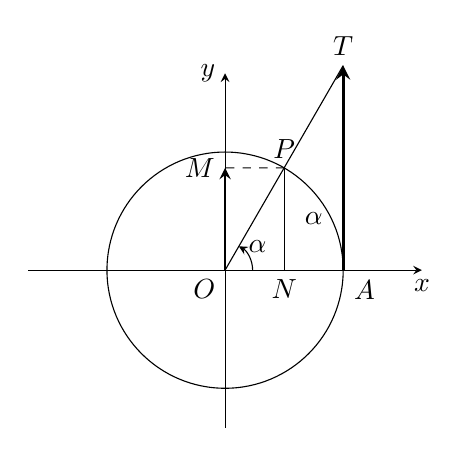
\begin{tikzpicture}[>=stealth]
\draw[->](-2.5,0)--(2.5,0)node[below]{$x$};
\draw[->](0,-2)--(0,2.5)node[left]{$y$};
\draw(0,0)node[below left]{$O$} circle(1.5);
\draw[->, very thick](1.5,0)node[below right]{$A$}--(60:3);
\draw(60:3)node[above]{$T$}--(0,0);
\draw(60:1.5)node[above]{$P$}--(1.5/2,0)node[below]{$N$};
\draw[->, thick](0,0)--(0,1.5/2*1.732)node[left]{$M$};
\draw[dashed](60:1.5)--(0,1.5/2*1.732);
\tkzDefPoints{1.5/0/A, 0.75/0/N, 0.75/1.3/P}
\tkzMarkRightAngle(A,N,P)
\draw[->](.35,0) arc (0:60:.35)node[right]{$\alpha$};
\node at (30:1.3){$\alpha$};
\end{tikzpicture}
\captionof*{figure}{(第14题)}
\end{minipage}

